\chapter{Implementation}\label{chap:Implementation}
This project was conducted in \textit{two} major phases:

First, I constructed a core mathematical theory for \textit{type slicing} and \textit{cast slicing} formalising what these ideas actually were and considered the changes to the system presented by Seidel et al. for the \textit{type error witnesses search procedure} to work in Hazel.  

Then, I implemented the theories, making it suitable for implementation and extending it to the majority of the Hazel language. Further, suitable deviations from the theory were made upon critical evaluation and are detailed throughout.

\section{Type Slicing Theory}\label{sec:TypeSlicingTheory}

I develop a novel method, \textit{type slicing}, as a mechanism to aid programmers in understanding \textit{why} a term has a given type via static means. Three slicing mechanism have been devised with differing characteristics, all of which associate terms with their typing derivation to produce a \textit{typing slices}. 

The first two criteria attempt to give insight on the structure of the typing derivations, and hence how types are decided. While the third criterion gives a complete picture of the regions of code which contribute to the a term's type.

I would like to stress that the second and third criterion were \textit{very challenging} to formalise, requiring non-obvious mathematical machinery: \textit{context typing slices} (\cref{sec:ContextTypingSlices}), \textit{checking contexts} (\cref{def:CheckingContext}), and \textit{type-indexed slices} (\cref{sec:TypeIndexedSlices}).

\subsection{Expression Typing Slices}\label{sec:ExpressionTypingSlices}
First, I introduce what \textit{slices} are in this context. The aim is to provide a formal representation of term \textit{highlighting}. 

\subsubsection{Term Slices}
A \textit{term slice} is a term with some sub-terms omitted. The omitted terms are those that are \textit{not} highlighted. For example if my slicing criterion is to \textit{omit terms which are typed as} \code{Int}, then the following expressions highlights as:

\[\hlcmaths[yellow!30]{(\lambda x: \code{Int}.\ \lambda y : \code{Bool}.}\ x\hlcmaths[yellow!30]{)(}1\hlcmaths[yellow!30]{)}\]


Omitted sub-terms are replaced by a \textit{gap} term, notated $\gap$. Representing the highlighted example above, we get the slice:
\[(\lambda x : \code{Int}.\ \lambda y : \code{Bool}.\ \gap)(\gap)\]

Similarly, this one can omit variable names and parts of types. We get a syntax specified in \cref{def:ExpressionSliceSyntax}, extending the Hazel core syntax from \cref{fig:syntax}: 
\begin{definition}[Term Slice Syntax]
\label{def:ExpressionSliceSyntax}
Pattern expression slices $p$:
\[p ::= \gap \mid x\]
Type slices $\upsilon$:\footnote{A \textit{type slice} is also used to refer to this whole mechanism. The overall theory is referred to \textit{typing slices} to distinguish from slices of type terms where ambiguous.}
\[\upsilon ::= \gap \mid \dyn \mid b \mid \upsilon \to \upsilon\]
Expression slices $\varsigma$:
\[\varsigma ::= \gap \mid  c \mid x \mid \lambda p : \upsilon.\ \varsigma \mid \lambda p.\ \varsigma \mid \varsigma(\varsigma) \mid \hole^u \mid \hole[\varsigma]^u \mid \varsigma : \upsilon\]
\end{definition}

We then have a \textit{precision} relation on term slices: $\varsigma_1 \sqsubseteq \varsigma_2$ meaning $\varsigma_1$ is less or equally precise than $\varsigma_2$. That is, $\varsigma_1$ matches $\varsigma_2$ structurally except that some sub-terms may be gaps. Full definition in appendix \textbf{ref appendix}. For example, see this precision chain:
\[\gap \sqsubseteq\gap + \gap\sqsubseteq 1 + \gap \sqsubseteq 1 + 2\]
Precision forms a partial order \cite{PartialOrder}, that is, a reflexive, antisymmetric, and transitive relation. Respectively:
\[\inference{}{\varsigma \sqsubseteq \varsigma} \quad \inference{\varsigma_1 \sqsubseteq \varsigma_2 & \varsigma_2 \sqsubseteq \varsigma_1}{\varsigma_1 = \varsigma_2} \quad \inference{\varsigma_1 \sqsubseteq \varsigma_2 & \varsigma_2 \sqsubseteq \varsigma_3}{\varsigma_1 \sqsubseteq \varsigma_3}\]
We also have a \textit{bottom} (least) element, $\gap \sqsubseteq \varsigma$ (for all $\varsigma$). This relation is trivially extended to include \textit{complete terms}\footnote{With no gaps.} $e$ which are \textit{top} elements of their respective chains: if $e \sqsubseteq \varsigma$ then $e = \varsigma$. Sometimes I refer to this relation as $\varsigma_1$ is a term slice \textit{of} $\varsigma_2$ iff $\varsigma_1 \sqsubseteq \varsigma_2$.

For any \textit{complete term} $t$, the slices of $t$ form a \textit{bounded lattice structure} \cite{Lattice}. That is, every pair $\varsigma_1, \varsigma_2$ has a \textit{join} $\varsigma_1 \sqcup \varsigma_2$ and \textit{meet} $\varsigma_1 \sqcap \varsigma_2$:
\begin{proposition}[Term Slice Bounded Lattice]
For any term $t$, the set of slices $\varsigma_1$ and $\varsigma_2$ of $t$ forms a bounded lattice:

\begin{minipage}{0.95\textwidth}
\begin{itemize}
\item The join, $\varsigma_1 \sqcup \varsigma_2$ exists , being an upper bound for $\varsigma_1, \varsigma_2$:
\[\varsigma_1 \sqsubseteq \varsigma_1 \sqcup \varsigma_2\qquad \varsigma_2 \sqsubseteq \varsigma_1 \sqcup \varsigma_2\]
And, any other slice $\varsigma \sqsubseteq t$ which is also an upper bound of $\varsigma_1, \varsigma_2$ is more or equally precise than the join:
\[\varsigma_1 \sqcup \varsigma_2 \sqsubseteq \varsigma\]
\item The meet, $\varsigma_1 \sqcap \varsigma_2$ exists, being a lower bound for $\varsigma_1, \varsigma_2$:
\[\varsigma_1 \sqcap \varsigma_2 \sqsubseteq \varsigma_1\qquad  \varsigma_1 \sqcap \varsigma_2 \sqsubseteq\varsigma_2\]
And, any other slice $\varsigma \sqsubseteq t$ which is also a lower bound of $\varsigma_1, \varsigma_2$ is less or equally precise than the meet:
\[ \varsigma \sqsubseteq\varsigma_1 \sqcup \varsigma_2\]
\item And the join and meet operations satisfy the absorption laws for any slice $\varsigma$:
\[\varsigma_1 \sqcap (\varsigma_1 \sqcup \varsigma_2) = \varsigma_1 \qquad \varsigma_1 \sqcup (\varsigma_1 \sqcap \varsigma_2) = \varsigma_1\]
And idempotent laws:
\[\varsigma_1 \sqcup \varsigma_1 = \varsigma_1 = \varsigma_1 \sqcap \varsigma_1\]
\item The lattice is bounded. That is, $\gap \sqsubseteq \varsigma \sqsubseteq t$.
\end{itemize}
\end{minipage}
\end{proposition}

Note that not every pair of slices has a join: consider $1$ and $2$. But, every pair does have a meet as for all $\varsigma_1, \varsigma_2$, $\gap \sqsubseteq \varsigma_1$ and $\gap \sqsubseteq \varsigma_2$.
 
\subsubsection{Typing Assumption Slices}
Expression typing is performed given a set of \textit{typing assumptions}. Therefore, in addition to a slice of expressions, we also desire a slice of the typing assumptions, to represent the \textit{relevant}\footnote{Relevant to the given criterion.} parts of the typing assumptions. Typing assumptions are \textit{partial functions} mapping variables to types notated $x : \tau$ (see \cref{sec:TypingJudgements}). 

Therefore, \textit{typing assumptions slices} can be represented by partial functions mapping variables to \textit{type slices}. That is, a typing assumption set is a slice of another if it maps \textit{no more} variables to \textit{at most} as specific types. The precision relation, $\sqsubseteq$, can be extended to typing assumptions by extensionality \cite{Extensionality} and using the subset relation:

\begin{definition}[Typing Assumption Slice Precision]
For typing assumption slices $\gamma_1, \gamma_2$. Where $\mathrm{dom}(f)$ is the set of variables for which a partial function $f$ is \textit{defined}:
\[\gamma_1 \sqsubseteq \gamma_2 \iff \mathrm{dom}(\gamma_1) \subseteq \mathrm{dom}(\gamma_2) \text{ and } \forall x \in  \mathrm{dom}(\gamma_1).\ \gamma_1(x) \sqsubseteq \gamma_2(x)\]
\end{definition}
Equally, joins and meet can be extended extensionality:
\begin{definition}[Typing Assumption Slice Joins and Meets]
For typing slices $\gamma_1, \gamma_2$, and any variable $x$:


\begin{minipage}{0.8\textwidth}
\begin{itemize}
\item If $\gamma_1(x) = \bot$ then $(\gamma_1 \sqcup \gamma_2)(x) = \gamma_2(x)$ and $(\gamma_1 \sqcap \gamma_2)(x) = \bot$. 
\item If $\gamma_2(x) = \bot$ then $(\gamma_1 \sqcup \gamma_2)(x) = \gamma_1(x)$ and $(\gamma_1 \sqcap \gamma_2)(x) = \bot$
\item Otherwise, $(\gamma_1 \sqcup \gamma_2)(x) = \gamma_1(x) \sqcup \gamma_2(x)$.
\end{itemize}
\end{minipage}
\end{definition}
Again, the slices $\gamma$ of complete typing assumptions $\Gamma$ form a bounded lattice. Similarly, not every pair of slices has a join, as not every type slice has a join: consider $x : \code{Int}$ and $x : \code{String}$.

\begin{proposition}[Typing Assumption Slices form Bounded Lattices]
For any typing assumptions $\Gamma$, the set of slices $\gamma$ of $\Gamma$ form a bounded lattice with bottom element of the empty function $\emptyset$ and top element $\Gamma$.
\end{proposition}
\subsubsection{Expression Typing Slices}
Finally, an \textit{expression typing slice}, $\rho$, is a pair, $\varsigma^\gamma$, of a term slice and a typing slice. Precision, joins and meets, can be extended pointwise to term typing slices with all the same properties:
\begin{definition}[Expression Typing Slice Precision]
For expression typing slices $\varsigma_1^{\gamma_1}$, $\varsigma_2^{\gamma_2}$:
\[\varsigma_1^{\gamma_1} \sqsubseteq \varsigma_2^{\gamma_2} \iff  \varsigma_1 \sqsubseteq \varsigma_2 \text{ and } \gamma_1 \sqsubseteq \gamma_2\]
\end{definition}
\begin{definition}[Expression Typing Slice Joins and Meets]
For expression typing slices $\varsigma_1^{\gamma_1}$, $\varsigma_2^{\gamma_2}$:
\[\varsigma_1^{\gamma_1} \sqcup \varsigma_2^{\gamma_2} = (\varsigma_1 \sqcup \varsigma_2)^{\gamma_1 \sqcup \gamma_2}\]
\[\varsigma_1^{\gamma_1} \sqcap \varsigma_2^{\gamma_2} = (\varsigma_1 \sqcap \varsigma_2)^{\gamma_1 \sqcap \gamma_2}\]
\end{definition}

For any pair of complete expressions $e$ and typing assumptions $\Gamma$, then the expression typing slices of these forms a bounded lattice.

\begin{proposition}[Expression Typing Slices for Bounded Lattices]
For any expression $e$ and typing assumption $\Gamma$, the set of expression typing slices $\varsigma^{\gamma}$ of $e^{\Gamma}$ forms a bounded lattice with bottom element $\gap^{\emptyset}$ and top element $e^{\Gamma}$.
\end{proposition}

The \textit{expression slices} can be \textit{type checked} under the \textit{type assumption slices} by replacing gaps $\gap$ by: holes of arbitrary metavariable $\hole^u$ in \textit{expressions}, fresh variables in \textit{patterns}, and the dynamic type in \textit{types}. This transformation $\type{\cdot}$ is stated formally in the appendix \textbf{(fig APPENDIX)}.

\begin{definition}[Expression Typing Slice Type Checking]
For expression typing slice $\varsigma^{\gamma}$ and type $\tau$. $\synthesis[\gamma]{e}{\tau}$ iff $\synthesis[\type{\gamma}]{\type{e}}{\tau}$ and $\analysis[\gamma]{e}{\tau}$ iff $\analysis[\type{\gamma}]{\type{e}}{\tau}$.
\end{definition}
\subsection{Context Typing Slices}\label{sec:ContextTypingSlices}
Next, some of an expression's type might be enforced by the surrounding \textit{context}. For example, the  type of the underlined expression below is enforced by the surrounding highlighted annotation:
\[\underline{(\lambda x. \hole^u )} \hlcmaths[yellow!30]{:  \code{Bool} \hlcmaths[yellow!30]{\to \code{Int}}}\]

\subsubsection{Contexts \& Context Slices}
\newcommand{\C}{\mathdcal{C}}
We represent these surrounding contexts by a \textit{term context} $\mathdcal{C}$. Which marks \textit{exactly one} sub-term as $\cmark$:
\begin{definition}[Contexts Syntax]
Pattern contexts -- mapping patterns to patterns:
\[\mathdcal{P} ::= \cmark \mid x\]
Type contexts -- mapping types to types: 
\[\mathdcal{T} ::= \cmark \mid \dyn \mid b \mid \mathdcal{T} \to \tau \mid \tau \to \mathdcal{T}\]
Expression contexts -- mapping patterns, types, or expression to expressions:\footnote{Note that $\C$ is also used for generic term contexts sometimes.}
\[\C ::=  \cmark \mid \lambda \mathdcal{P} : \tau.\ e \mid \lambda x : \mathdcal{T}.\ e \mid \lambda x : \tau.\ \C \mid \lambda \mathdcal{P}.\ e \mid \lambda x.\ \C \mid \C(e) \mid e(\C) \mid e : \mathdcal{T} \mid \C : \tau\]
\end{definition}

Where $\C\{e\}$ substitutes expression $e$ for the mark $\cmark$ in $\C$, the result of this is necessarily an expression. Similarly for pattern and type contexts $\mathdcal{P}, \mathdcal{T}$ whose substitutions return patterns and types. Additionally, contexts are \textit{composable}: substituting a context into a context, $\C_1\{\C_2\}$ produces another valid context when the domain of $\C_1$ is from expressions. Notate this by $\C_1 \circ \C_2$. From here on I notate all contexts like functions, specifying their domain and co-domain where appropriate: $\C : \code{Typ} \to \code{Exp}$ for example.


\newcommand{\Cs}{\mathdcal{c}}
\newcommand{\p}{\mathdcal{p}}
Then, contexts can be extended to slices, $\Cs$, analogously to the previous section. However, the precision relation $\sqsubseteq$ is defined differently, requiring that the mark $\cmark$ must remain in the same position in the structure. For example $\cmark(\gap) \sqsubseteq \cmark(1)$, but $\cmark \not \sqsubseteq \cmark(1)$. This can be concisely defined by \textit{extensionality}:

\begin{definition}[Context Precision]\label{def:ContextPrecision}
If $\Cs : \code{X} \to \code{Y}$ and $\Cs' : \code{X} \to \code{Y}$ are context slices, then $\Cs' \sqsubseteq \Cs$ if and only if, for all terms $t$ of class $\code{X}$, that $\Cs'\{t\} \sqsubseteq \Cs\{t\}$.
\end{definition}

Again, we refer to a context slice $\Cs'$ \textit{of} $\Cs$ as one satisfying that $\Cs' \sqsubseteq \Cs$.

We also get that filling contexts preserves the precision relations both on term slices \textit{and} context slices:\footnote{The conjectures are heavily suspected but not formally proven in the appendix.}
\begin{conjecture}[Context Filling Preserves Precision]
For context slice $\Cs : \code{X} \to \code{Y}$ and term slice $\varsigma$ of class \code{X}. Then if we have slices $\varsigma' \sqsubseteq \varsigma$, $\Cs' \sqsubseteq \Cs$ then also $\Cs'\{\varsigma'\} \sqsubseteq \Cs\{\varsigma\}$.
\end{conjecture}

Joins and meets can be defined via extensionality:
\begin{definition}[Context Slice Joins \& Meets]
For context slices $\Cs_1 : \code{X} \to \code{Y}$ and $\Cs_2 : \code{X} \to \code{Y}$ and any term $t$ of class \code{X}:
\[(\Cs_1 \sqcup \Cs_2)\{t\} = \Cs_1\{t\} \sqcup \Cs_2\{t\}\]
\[(\Cs_1 \sqcap \Cs_2)\{t\} = \Cs_1\{t\} \sqcap \Cs_2\{t\}\]
\end{definition}

Again, these form a lattice:
\begin{proposition}[Context Slices form Bounded Lattices]
For any context $\C$, the set of slices $\Cs$ of $\C$ form a bounded lattice with bottom element of the \textit{purely structural context}\footnote{With the $\cmark$ is the \textit{same position} but every other sub-term being a $\gap$. Defined in appendix.} and top element $\C$.
\end{proposition}

\subsubsection{Typing Assumption Contexts \& Context Slices}
The accompanying notion of a \textit{typing assumption slice} can be extended to \textit{functions on typing assumptions}. This function represents what typing assumptions need to be \textit{added}, or can be \textit{removed} when typing an expression $e$ and within it's context slice.

\newcommand{\F}{\mathdcal{F}}
\newcommand{\f}{\mathdcal{f}}
\begin{definition}[Typing Assumption Contexts \& Slices]
A typing assumption context $\F$ is a function from typing assumption to typing assumptions. A typing assumption context slice $\f$ is a function from typing assumption slices to typing assumption slices.
\end{definition}

Functions can be composed and a precision partial order can also be defined via extensionality:
\begin{definition}[Typing Assumption Context Slice Precision]\label{def:FunctionPrecision}
If $\f'$ and $\f$ are typing assumption context slices, then $\f' \sqsubseteq \f$ if and only if, for all typing context slices $\gamma$, that $\f'(\gamma) \sqsubseteq \f(\gamma)$.
\end{definition}
Again, such functions are monotone:
\begin{conjecture}[Function Application Preserves Precision]
For typing assumption slice $\gamma$ and typing assumption context slice $\f$. Then if we have slices $\gamma' \sqsubseteq \gamma$, $f' \sqsubseteq f$ then also $f'(\gamma') \sqsubseteq f(\gamma)$.
\end{conjecture}
Joins and meets are also defined extensionally:
\begin{definition}[Typing Assumption Context Slice Joins \& Meets] For typing assumption context slices $\f_1$ and $\f_2$ and any typing assumption slice $\gamma$:
\[(\f_1 \sqcup \f_2)(\gamma) = \f_1(\gamma) \sqcup \f_2(\gamma)\]
\[(\f_1 \sqcap \f_2)(\gamma) = \f_1(\gamma) \sqcap \f_2(\gamma)\]
\end{definition}

\begin{conjecture}[Typing Assumption Context Slices form Bounded Lattices]
For any typing assumption context $\F$, the set of slices $\f$ of $\F$ form a bounded lattice with bottom element being the constant function to the empty typing assumption function and top element $\F$.
\end{conjecture}

As usual, not all joins exist: if the assumption context slices map the slices to inconsistent typing assumption slices. 
\subsubsection{Context Typing Slices}
Finally, an \textit{expression context typing slice}, $\p$, is a pair, $\Cs^\f$, of an expression context slice and a typing assumption context slice. Precision, composition, application, joins and meets, can be extended pointwise to term typing slices with all the same properties:
\begin{definition}[Expression Context Typing Slice Precision]
For expression context typing slices $\Cs_1^{\f_1}$, $\Cs_2^{\f_2}$:
\[\Cs_1^{\f_1} \sqsubseteq \Cs_2^{\f_2} \iff  \Cs_1 \sqsubseteq \Cs_2 \text{ and } \f_1 \sqsubseteq \f_2\]
\end{definition}
\begin{definition}[Expression Context Typing Slice Composition \& Application]
For expression context typing slices $\Cs^{\f}$, $\Cs'^{\f'}$, and expression typing slices $\varsigma^{\gamma}$:
\[\Cs^{\f} \circ \Cs'^{\f'} =  (\Cs \circ \Cs')^{\f \circ \f'}\]
\[\Cs_1^{\f_1}\{\varsigma^{\gamma}\} =  \Cs_1\{\varsigma\}^{\f_1(\gamma)}\]
\end{definition}
\begin{definition}[Expression Context Typing Slice Joins and Meets]
For expression typing slices $\Cs_1^{\f_1}$, $\Cs_2^{\f_2}$:
\[\Cs_1^{\f_1} \sqcup \Cs_2^{\f_2} = (\Cs_1 \sqcup \Cs_2)^{\f_1 \sqcup \f_2}\]
\[\Cs_1^{\f_1} \sqcap \Cs_2^{\f_2} = (\Cs_1 \sqcap \Cs_2)^{\f_1 \sqcap \f_2}\]
\end{definition}

For any pair of expressions contexts $\C$ and typing assumption contexts $\F$, then the expression typing slices of these forms a bounded lattice.

\begin{proposition}[Expression Context Typing Slices form Bounded Lattices]
For any expression context $\C$ and typing assumption context $\F$, the set of expression context typing slices $\Cs^{\f}$ of $\C^{\F}$ forms a bounded lattice with bottom element, the purely structural context and the function to the empty typing assumptions, and top element $e^{\Gamma}$.
\end{proposition}

\subsection{Type-Indexed Slices}\label{sec:TypeIndexedSlices}
Tagging slices by their type and allowing decomposition into sub-slices for each part of the type is required for \textit{cast slicing} and useful in calculating slices according to \textit{analysis slices} and \textit{contribution slices} criteria. For example consider the same context slice:
\[\underline{(\lambda x. \hole^u )} \hlcmaths[yellow!30]{:  \code{Bool} \hlcmaths[yellow!30]{\to \code{Int}}}\]
This context slice would be tagged with type $\code{Bool} \to \code{Int}$ and the respective sub-slice considering only the return type would omit the \code{Bool} term:
\[\underline{(\lambda x. \hole^u )} \hlcmaths[yellow!30]{:}  \code{Bool} \hlcmaths[yellow!30]{\to \code{Int}}\]

This section will only consider \textit{context slices}, but term slices are type-indexed in exactly the same way. By extending the class of possible contexts, an expression slice can be considered as a \textit{terminal context}\footnote{Being a terminal morphism when thinking of morphisms in a category.} taking any input to the expression slice.\footnote{These will be used interchangeably from now on.}
\begin{definition}[Term Slices as Terminal Context Slices]
A terminal context slice for a term typing slice $\rho$ is a context typing slice $\p$ such that for every context typing slice $\p'$ and expression typing slice $\rho'$:
\[\p \circ \p' = \p \text{ and } \p\{\rho'\} = \rho\]
\end{definition}

The main property that we want these indexed-slices to maintain is that a slice can be \textit{reconstructed} from their sub-parts. \textit{Joining} the sub-slices should produce the slice for the entire type. As not every slice can be joined, we can pair sub-slices with contexts which place the two sub-slices inside the same structure, making them join-able.

\renewcommand{\S}{\mathdcal{S}}
\newcommand{\s}{\mathdcal{s}}
\begin{definition}[Type-Indexed Context Typing Slices]
Syntactically defined: 
\[\S ::= \p \mid \p * \S \to \p * \S\] 
With any $\S$ only being valid if it has a full slice. The full slice of $\S$ is notated $\overline{\S}$ and defined recursively:
\[\overline{\p} = \p\]
\[\overline{\p_1 * \S_1 \to \p_2 * \S_2} = \p_1 \circ \overline{\S_1} \sqcup \p_2 \circ \overline{S_2}\]
\end{definition}
Then left \textit{(incremental)} composition and right \textit{(global)} composition can be defined, by composing at the upper type constructor or at the leaves respectively:
\begin{definition}[Type-Indexed Context Typing Slice Composition]
For type-indexed context typing slices $\S$ and $\S'$.  If $\S = \p$ and $\S' = \p'$:\footnote{In shorthand, the overline for a base type slice is often omitted.}
\[\p' \circ \p = \overline{\p'} \circ \overline{\p}\qquad \p \circ \p' = \overline{\p} \circ \overline{\p'}\]
If $\S = \p$ and $\S' = \p_1' * \S_1' \to \p_2' * \S_2'$:\footnote{In shorthand, brackets will be omitted.}
\[S \circ \S' = (\p \circ p_1') * \S_1' \to (\p \circ \p_2') * \S_2'\]
If $\S = \p_1 * \S_1 \to \p_2 * \S_2$:
\[\S \circ \S' = \p_1 * (\S_1 \circ \S') \to \p_2 * (\S_2 \circ \S')\]
\end{definition}

This definition stems from it representing regular context typing slice composition over it's full slices.
\begin{proposition}[Type-Indexed Composition Preserves Full Slice Composition]
For type-indexed slices $\S$ and $\S'$: 
\[\overline{\S \circ \S'} = \overline{\S} \circ \overline{\S'}\]
\end{proposition}


\subsection{Criterion 1: Synthesis Slices}
\label{sec:SynthesisSlices}

The first slicing method aims to concisely explain why an expression \textit{synthesises} a type. It omits all  sub-terms which analyse against a type retrieved from synthesising some other part of the program. For example, the following term synthesises a $\code{Bool} \to \code{Bool}$ type, and the variable $x : \code{Int}$ and argument are irrelevant:

\[\hlcmaths[yellow!30]{(\lambda} x: \code{Int}\hlcmaths[yellow!30]{.\ \lambda y : \code{Bool}.\ y)(}1\hlcmaths[yellow!30]{)}\]

\begin{definition}[Synthesis Slices]
For a synthesising expression, $synthesis{e}{\tau}$. A synthesis slice is an expression typing slice $\varsigma^{\gamma}$ of $e^\Gamma$ which also synthesises $\tau$, that is, $\synthesis[\type{\gamma}]{\type{\varsigma}}{\tau}$.
\end{definition}
\begin{proposition}[Minimum Synthesis Slices]
A minimum synthesis slice of $e^\Gamma$ is a synthesis slice $\rho$ such that any other synthesis slices $\rho'$ are at least as specific, $\rho \sqsubseteq \rho'$. This minimum always uniquely exists.
\end{proposition}

These slices can be defined via a typing judgement $\synthesisslice{e}{\tau}{\S}$, meaning $\S$ is the type-indexed synthesis slice of $e^\Gamma$ synthesising $\tau$. The non-indexed version can be retrieved by $\overline{\S}$. This judgement mimics the Hazel typing rules, while omitting portions of the program which are \textit{type analysed} from the slice.  

For example, when encountering application, the type of the function is synthesised purely by the function itself, so the argument can be omitted:
\[\inference{\synthesisslice{e_1}{\tau_1}{\S_1} & \tau_1 \funmatch \tau_2 \to \tau & \S_1 \funmatch \S_2 \to \S & \analysis{e_2}{\tau_2}}{\synthesisslice{e_1(e_2)}{\tau}{\S}}\]
Where function matching $\funmatch$ is extended to slices by eagerly applying the contexts paired with the slice sub-parts if applicable:
\[\Cs \funmatch \Cs \to \Cs\]
\[\Cs_1 * \S_1 \to \Cs_2 * \S_2 \funmatch \Cs_1 \circ \S_1 \to \Cs_2 \circ \S_2\]
This approach correctly calculates the synthesis slices.
\begin{conjecture}[Correctness]
\label{conj:SynthesisSliceCorrectness}
If $\synthesis{e}{\tau}$ then:
\begin{itemize}
\item $\synthesisslice{e}{\tau}{\rho}$ where $\rho = \varsigma^\gamma$ with $\synthesis[\gamma]{\varsigma}{\tau}$.
\item For any $\rho' = \varsigma'^{\gamma'} \sqsubseteq e^\Gamma$ such that $\synthesis[\gamma']{\varsigma'}{\tau}$ then $\rho \sqsubseteq \rho'$.
\end{itemize}
\end{conjecture}

\subsection{Criterion 2: Analysis Slices}\label{sec:AnalysisSlices}
A similar idea can be devised for analysis slices. Essentially, we do the opposite of \textit{criterion 1} and omit sub-terms where \textit{synthesis} was used. The objective is to show \textit{why} a term is required to be checking against a type.

The way to represent these are \textit{context slices}. It is the terms immediately \textit{around} the sub-term where the type checking is enforced. For example, when checking this annotated term:
\[(\lambda x. \hole^u) : \code{Bool} \to \code{Int}\]
The \textit{inner hole term} $\hole^u$ (underlined) is required to be consistent with \code{Int} due to the annotation. Therefore, the hole's analysis slice will be:
\[\hlcmaths[yellow!30]{(\lambda} x\hlcmaths[yellow!30]{.} \underline{\hole^u} \hlcmaths[yellow!30]{) : } \code{Bool} \hlcmaths[yellow!30]{\to \code{Int}}\]
Intuitively, this means that the \textit{contextual} reason for $\hole^u$ to be required to be an \code{Int} is: that it is within a function which the annotation enforced to check against $\code{Bool} \to \code{Int}$, of which only the return type ($\code{Int}$) is relevant.

In other words, if the context slice was type synthesised, then the marked term would still be \textit{required} to check against \code{Int}. However, the overall synthesised type may differ.\footnote{The previous example would synthesis $\dyn \to \code{Int}$ as opposed to $\code{Bool} \to \code{Int}$.}


\subsubsection{Checking Context}
For this, we only want to consider the smallest context scope\foornote{The \textit{size} of the context around the marked term.} that enforced the type checking. For example, the below term has 3 annotations, but only the inner one enforces the \code{Int} type on the integer 1:
\[\underline{1} \hlcmaths[yellow!30]{: \code{Int}} : \dyn : \code{Bool}\]
I refer to this minimum context scope as the \textit{checking context}, and checking contexts will always synthesise a type. Another way for types to be enforced is via application. The integer argument's type is enforced by the annotation on the function:
\[\hlcmaths[yellow!30]{(\lambda} x \hlcmaths[yellow!30]{: \code{Int}.}\ \hole^u\hlcmaths[yellow!30]{)(}\underline{1}\hlcmaths[yellow!30]{)}\]


\begin{definition}[Checking Context]
\label{def:CheckingContext}
For term $e$ checking against $\tau$: $\analysis[\Gamma]{e}{\tau}$. A checking context for $e$ is an expression context $\C$ and typing assumption context $\F$ such that: 
\begin{itemize}
\item $\synthesis[\F(\Gamma)]{\C\{e\}}{\tau'}$ for some $\tau'$.
\item The above derivation has a sub-derivation $\analysis[\Gamma]{e}{\tau}$.
\end{itemize}
\end{definition}
\begin{definition}[Minimally Scoped Checking Context]
For a derivation $\analysis[\Gamma]{e}{\tau}$, it's minimally scoped expression checking context is a checking context of $e$ such that no sub-context is also a checking context.
\end{definition}

All possible minimally scoped checking contexts can be constructed syntactically via rules. This coincides with the definition above, but is more amenable to performing proofs on. Given in the appendix \textbf{ref}.

If $e'$ is a sub-term in a synthesising expression $e$, there will be a unique minimally scoped checking context $\C$ which matches the structure of the original term and typing assumption context $\F$ mapping the context used to type $e'$ to the context used to synthesise $e'$ in it's checking context. 
\begin{proposition}[Checking Context of a Sub-term in a Derivation]
If derivation $\synthesis{e}{\tau}$ contains a analysis sub-derivation $\analysis[\Gamma']{e'}{\tau'}$ for sub-term $e'$. Then there is a unique minimally scoped context $\C$ for $e'$ and typing assumption context $\F$ for $\Gamma'$ such that:
\begin{itemize}
\item $\C\{e'\}$ is a sub-term of $e$, or is $e$ itself.
\item Derivation $\synthesis{e}{\tau}$ contains a sub-derivation for $\synthesis[\F(\Gamma')]{\C\{e'\}}{\tau''}$, or is the derivation itself: $\tau'' = \tau, \C\{e'\} = e,$ and $\F(\gamma') = \Gamma$.
\end{itemize}
\end{proposition}

This checking context of a sub-term in a derivation can be calculated during type checking of the term. These checking contexts are what is actually useful for explaining type analysis in a \textit{specific} program.

But, more generally, analysis slices are then a slice of any \textit{minimally scoped checking context}.

\begin{definition}[Analysis Slice]\label{def:analysisslice}
For a term $e$ analysing against $\tau$: $\analysis{e}{\tau}$, and a checking context $\C^\F$ for $e$. An analysis slice is a slice, $\Cs^\f$, of $\C^\F$ which is also a checking context for $e$. That is:
\begin{itemize}
\item $\synthesis[\f(\Gamma)]{\Cs\{e\}}{\tau'}$ for some $\tau'$.
\item The above derivation has a sub-derivation for $\analysis{e}{\tau}$. 
\end{itemize}
\end{definition}

The \textit{minimum analysis slice} is just the minimum under the precision ordering $\sqsubseteq$. And it must be unique:

\begin{conjecture}[Minimum Analysis Slices]\label{conj:AnalysisSliceUniqueness}
The minimum analysis slice analysing $e$ in a checking context $\C^\F$ is an analysis slice $\p$ such that for any other any other analysis slice $\p'$ is at least as specific, $\p \sqsubseteq \p'$. This minimum always uniquely exists.
\end{conjecture}

This can again be represented by a judgement read as, \textit{$e$ which type checks against $\tau$ in checking context $\C$ has (type-indexed) analysis slice $\S$}:\footnote{Again, non-indexed version retrieved by $\overline{\S}$.}
\[\analysisslice{\C}{e}{\tau}{\p}\]

There are two situations which enforce \textit{checking contexts}, of which application is most interesting, calculating the minimum indexed synthesis slice of the context and retrieving just the sub-slice relevant to typing the \textit{argument}:\footnote{Note that $e_1$ synthesises $\tau_2$ exactly here. Contribution slices consider situations involving subsumption which may synthesise different but consistent types.}

\[\inference{\synthesisslice{e_1}{\tau_1}{\S_1} & \tau_1 \funmatch \tau_2 \to \tau & \S_1 \funmatch \S_2 \to \S & \analysis{e_2}{\tau_2}}{\analysisslice{\C}{e_2}{\tau_2}{(\Cs^\f \mapsto \Cs(\cmark)^\f) \circ S_1}}\]
Where $(\Cs^\f \mapsto \Cs(\cmark)^\f)$ maps the outer expression slices to context slices matching the input checking context. \textbf{(add this `two-hole-context' to the type-indexed slice section, maybe make type-indexed expression slices explicit.} 

This definition does indeed find the minimum analysis slice:
\begin{conjecture}[Correctness]\label{conj:AnalysisSliceCorrectness}
If $\C$ is a checking context for $e$ and $\analysis{e}{\tau}$. Then $\analysisslice{\C}{e}{\tau}{\S}$ and $\S$ is the minimum analysis slice of $e$.
\end{conjecture}

\subsection{Criterion 3: Contribution Slices}
\label{sec:ContributionSlices}
This criterion aims to highlight all regions of code which \textit{contribute} to the given type (either synthesised or analysed). Where \textit{contribute} means that there exists a type that if the sub-term changed it's type to, then the overall term would also change type, or would become ill-typed. Importantly, we also consider \textit{contexts} for expression which are analysed, again considering any component terms which having their type changed would result in an error when trying to analyse against the type. For example in the following term:

\[(\lambda f: \code{Int} \to \dyn.\ f(1))\underline{(\lambda x : \code{Int}.\ x)}\]
The terms which \textit{contribute} to the \textit{underlined} lambda term checking successfully against $\code{Int} \to \dyn$ is everything \textit{except} the $x$ term, while context slice is just the annotation (and required structural constructs). Highlighting related to synthesis will be a darker shade:
\[\hlcmaths[yellow!30]{(\lambda} f\hlcmaths[yellow!30]{: \code{Int} \to \dyn}.\ f(1)\hlcmaths[yellow!30]{)}\underline{\hlcmaths[yellow!70]{(\lambda} x \hlcmaths[yellow!70]{: \code{Int}.}\ x\hlcmaths[yellow!70]{)}}\]

Notice that, in any typing derivation the only sub-terms which \textit{can} have their type changed without causing the rule to no longer apply are those which use type \textit{consistency}.\footnote{Note that this logic does \textit{not} extend to globally inferred languages.} The only such rule is \textit{subsumption}. Further, the only time a term could be changed to \textit{any} type and still remain valid is when it is checked for consistency with the dynamic type $\dyn$.

Therefore, this criterion just \textit{omits all dynamically annotated regions} of the program.\footnote{But does not omit the dynamic annotations themselves.} And, the contextual part of the slices are just \textit{analysis slices}.

\begin{definition}[Contribution Slices]\label{def:ContributionSlice}
For $\synthesis{e}{\tau}$ containing sub-derivation $\analysis[\Gamma']{e'}{\tau'}$ with checking context $\C$.

A \textit{contribution slice} of $e'$ is an \textit{analysis slice} for $e'$ in $\C$ paired with an expression typing slice $\varsigma^\gamma$ such that:
\begin{itemize}
\item $\varsigma$ is a slice of $e'$, that $\varsigma \sqsubseteq e'$.
\item Under restricted typing context $\gamma$, that $\varsigma$ checks against any $\tau'_2$ at least as precise as $\tau'$:\footnote{Essentially, sub-terms that check against $\dyn$ also synthesise $\dyn$. Defined this way to include the case of unannotated lambdas (which do not synthesise).}
\[\forall \tau'_2.\ \tau' \sqsubseteq \tau'_2 \implies \analysis[\gamma]{e'}{\tau'_2}\]
\end{itemize}
A contribution slice for a sub-term $e''$ involved in sub-derivation $\synthesis[\Gamma'']{e''}{\tau''}$ where $e'' \neq e'$ is an expression typing slice $\varsigma''^{\gamma''}$ which also synthesises $\tau''$ under $\gamma''$, that $\synthesis[\gamma'']{\varsigma''}{\tau''}$. Further, any sub-term of $e''$ which has a contribution slice of the above variety, is replaced inside $\varsigma$ by that corresponding expression typing slice.
\end{definition} 
The synthetic parts of these slices can be calculated in exactly the same way as synthesis slices, except now also considering the \textit{subsumption} rule. The analytic parts are regular analysis slices.

The subsumption rule synthesises a type for some term, then checks consistency with the checked type. This is where the dynamic portions can be omitted, to give a contribution slice for the checked term. Representing contribution slices with the judgement $\contributionslice{e}{\tau}{\S}$ and $\contributionanalysisslice{\C}{e}{\tau}{\S_e}{\S_c}$, where $\S_e$ is the expression slice part and $\S_c$ is the contextual part:

\[\inference{\contributionslice{e}{\tau}{\S_s} & \tau \sim \tau' & \analysisslice{\C}{e}{\tau'}{\S_c}}{\contributionanalysisslice{\C}{e}{\tau'}{\mathrm{static}(\S_c, \S_s)}{\S_c}}\]
Where static is takes omits the \textit{right} (synthetic) slice parts where \textit{left} (analytic) slice is a leaf but the right is not. As the types are consistent, these leaves will be the unknown type. This means that portions of the synthetic part of the slice which match against $\dyn$ will be omitted: \textbf{SHOW A DIAGRAM}
\[\mathrm{static}(\p, \p') = \p'\]
\[\mathrm{static}(\p, \_ \to \_) = \gap^\emptyset\]
\[\mathrm{static}(\Cs_1 * \S_1 \to Cs_2 * \S_2,\ \Cs_1' * \S_1' \to Cs_2' * \S_2') = \Cs_1 * \mathrm{static}(\S_1, \S_1') \to \Cs_2' * \mathrm{static}(\S_2, \S_2')\]

\newcommand{\s}{\mathdcal{s}}
\begin{figure}[h]
\[\inference[\tiny SConst]{}{\synthesissliceindexed{c}{b\mid c}} \quad
\inference[\tiny SVar]{x : \tau \in \Gamma}{\synthesissliceindexed{x}{\mathrm{map}{(x^{\{x:\tau\}}, \tau)}}}\]
\[ 
\inference[\tiny SFun]{s_1 = (\gap : \cmark)\circ \mathrm{annot}(\tau_1) &\synthesissliceindexed[\Gamma,x:\tau_1]{e}{s_2}\\ s_2 = i_2 \mid \varsigma^\gamma & x \match{\gamma} p}{\synthesissliceindexed{\lambda x:\tau_1.\ e}{(\lambda \cmark.\ \gap) \circ s_1 \to (\lambda p : \tau_1.\ \cmark) \circ s_2 \mid (\lambda p : \tau_1.\ \varsigma)^{\gamma\backslash x:\tau_1}}}\]
\textbf{TODO: UPDATE THIS FIGURE, move to appendix!!}
\[\inference[\tiny SApp]{\synthesissliceindexed{e_1}{s_1} & s_1 \funmatch s_2 \to s \\ \analysissliceindexed{e_2}{s_2(\cmark)}{s_2'}}{\synthesissliceindexed{e_1(e_2)}{\text{app}(s_2')}}\]
 
\[\inference[\tiny SEHole]{}{\synthesissliceindexed{\hole^u}{\dyn \mid \hole^u}} \quad \inference[\tiny SNEHole]{\synthesissliceindexed{e}{\p\{i \mid \varsigma^\gamma\}}}{\synthesissliceindexed{\hole[e]^u}{\dyn \mid {\hole[\varsigma]^u}^\gamma}}\]
\[\quad 
\inference[\tiny SAsc]{c = \cmark : \text{annot}(\tau) & \analysissliceindexed{e}{\s}{s}}{\synthesis{e : \tau}{\mathrm{app}(s)}}\]

\[\inference[\tiny AFun]{\s \funmatch \s_1 \to \s_2\\ \analysissliceindexed[\Gamma, x:\type{\s_1}]{e}{\s_2 \circ (\lambda x.\ \cmark)}{s_2}}{\analysissliceindexed{\lambda x.e}{\s}{\s_1\{\lambda \gap. \gap\} \to s_2}}\] 
\[\inference[\tiny ASubsume]{\synthesissliceindexed{e}{s}\\ \type{s} \sim \type{\s}}{\analysissliceindexed{e}{\s}{\bigsqcup\mathrm{static}(\type{\s}, s)}}\]
\caption{Contribution Slices}
\label{fig:ContributionSliceRules}
\end{figure} 


\subsection{Type-Indexed Slicing Context}
\label{sec:TypeSliceContext}
It seems natural to extend the typing context to become a type-indexed slicing context. Then, when accessing typing assumptions via variable references, the slice information which derived this type can be revealed. But, as no context is propagated, the slices would have no .

\section{Cast Slicing Theory}\label{sec:CastSlicingTheory}
\textbf{This section is not written yet, but will be very short... The only addition is cast dependence, which is literally just a partial order on casts through dynamics.}

Fairly trivial, just treat tag types in casts with their slices and decompose accordingly.

The idea of it being a minimal expression typing slice producing the same cast doesn't really work here due to dynamics. Explore the maths of this. Either way, it is a useful construct in practice. Exploring this in more detail, looking at \textit{dynamic program slicing} could be a good future direction.

\textbf{Mention and compare with blame tracking?}

\subsection{Indexing Slices by Types}


\subsection{Elaboration}
All casts inserted come from type checking, so can be sliced.

\subsection{Dynamics}
Ground type casts will be added, but their addition is purely technical and we can treat their reasoning to just be extracting the relevant portion of the original non-ground type.

\subsection{Cast Dependence}
\label{sec:CastDependence}
This in combination with the indexed slices could have some nice mathematical properties.

Though, these would need to retrieve information about parts of slices that were lost when decomposing slices. i.e. when a slice $\tau_1 \to \tau_2$ extracts the argument type $\tau_2$, the slicing criteria lose track of the original lambda binding. A way to reinsert these bindings such that we get a minimal term which \textit{Evaluates to the same cast} e.g. But this will have lots of technicalities with correctly tracking the restricted contexts $\gamma'$ for closures (i.e. functions returning functions which have been applied once). \textbf{TALK ABOUT THIS IN THE FURTHER DIRECTIONS SECTION.}

\section{Type Slicing Implementation}\label{sec:TypeSlicingImplementation}
Here I detail how the theories above were adapted to produce an implementation for Hazel.
\subsection{Hazel Terms}
\label{sec:HazelTerms}
Hazel represents its abstract syntax tree (AST) \textbf{(cite)} in a standard way by creating a mutually recursive algebraic data-type (\textbf{cite}). 

Terms are classified into similar groups as described in the calculus (see \cref{sec:HazelSyntax}), though combining external and internal expressions, and adding \textit{patterns}:
\begin{itemize}
\item \textbf{Expressions}: The primary encompassing term including: constructors\footnote{The basic language constructs: integers, lists, labelled tuples etc. Also, user-defined constructors via sum types.}, holes, operators, variables, let bindings, functions \& closures, type functions, type aliases, pattern match expressions, casts, explicit fix\footnote{Fixed point combinator for recursion.} expression.
\item \textbf{Types}: Unknown type\footnote{Either dynamic type, or a type hole.}, base types, function types, product types, record types, sum types, type variables, universal types, recursive types.
\item \textbf{Patterns}: Destructuring constructs for bindings, used in functions, match statements, and let bindings, including: Holes, variables (to bind values to), wildcard, constructors, annotations (enforcing type requirements on bound variables). 
\item \textbf{Closure Environments}: a closure mapping variables to their assigned values in it's syntactic context.
\end{itemize}

For example \cref{fig:tupletermstructure} shows a let binding expression whose binding is a tuple pattern (in blue) binding two variables \code{x}, \code{y} annotated with a type (in purple).

\begin{figure}[h]
\center
\includegraphics[width=0.75\textwidth]{Media/Figures/tuple_term_structure}
\caption{Let binding a tuple with a type annotation.}
\label{fig:tupletermstructure}
\end{figure}

Every term (and sub-term) is annotated with an \textit{identifier} (ID, \code{Id.t}) in the AST which refers back to the syntax structure tree. In a sense, this is the equivalent of \textit{code locations}, but Hazel is edited via a structure editor. 
\subsection{Type Slice Data-Type}\label{sec:TypeSliceDataType}
I detail here \textit{how} and \textit{why} I implement type slices for Hazel.

\subsubsection{Expression slices as ASTs}

Directly storing expression slices directly as ASTs is both \textit{space and time inefficient}. The AST type is a persistent data structures \cite[ch. 2]{PurelyFunctionalDataStructures}, meaning that any update to the tree will retain both the old and updated tree. All nodes on the path to the updated sub-tree must be copied; for example, \cref{fig:PersistentTrees} shows how a node G (in blue) can be sliced off from the tree while the old tree (in black) and the new tree (in red) both persist and share some unmodified nodes structurally. Expression slices do exactly this slicing operation extensively, so would require significant copying.
\begin{figure}[h]
\center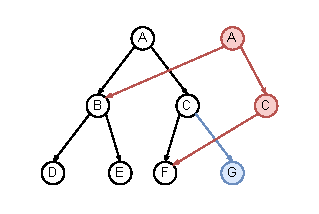
\includegraphics[width=0.75\textwidth]{Media/Figures/persistenttree}
\caption{Persistent Tree}
\label{fig:PersistentTrees}
\end{figure}

There are ways to partially avoid this, for example the \textit{Zipper} data structure represents trees by from the perspective of a \textit{cursor} node rather than the \textit{root}. The part of the tree above the cursor is stored as an \textit{upside-down}. This allows the cursor to be 

We can derive an analogous \textit{one-hole context} type for the AST by \textit{differentiating} it's type \cite{OneHoleContext, TypeDerivatives}. 


\textbf{Zippers only useful if we need access to the parent node which cannot just be done by passing down info.}

However, we still have to copy nodes when shifting the cursor; during type-checking all nodes will be visited by the cursor so we would get at least a \textit{doubling} in space used. Additionally, converting a zipper back into a tree would take linear time\footnote{In the depth of the cursor.} and still require copying the path to the cursor as before.\footnote{Still advantageous as it delays the copying only for when the slice is actually \textit{used} in a way that requires this conversion. UI for slices would still work directly on the zipper structure without copying.} 

\begin{figure}[h]
\textbf{Produce Tikz Diagram Here.}
\caption{Tree Zipper}
\label{fig:PersistentZipper}
\end{figure}


\textbf{NOTE: Actually the below might be inaccurate, I think I'm confusing myself with persistence. I think I could actually space-efficiently construct contextual and synthetic slices.}

\textbf{Either way, there is opportunity to speak about persistence with how type slices are combined and decomposed and how they overlap. etc. ?}

\textbf{The benefits of unstructured slices being more flexible apply either way. Plus, I don't actually need the slice structure for highlighting terms. Plus ids take up less space by a constant factor anyway.}

\subsubsection{Unstructured Code Slices}
\label{sec:UnstructuredSlices}
With this in mind, given that the structure of expression slices does not actually matter for highlighting\footnote{Only matters for type checking slices, which always succeeds by design.}, I represent slices indirectly by these IDs in an \textit{unstructured} list, referred to now as a \textit{code slice} (\code{code_slice} type).

 Additionally, this has the side effect of allowing more \textit{granular} control over slices, as they now need not conform with the structure of expressions which is taken advantage of to reduce slice size, \textbf{(ref to section discussing this + evaluation)}.

Equally, the typing assumption slices are only required for formal type checking, however I maintain these is code slices to allow for different UI styling of slices originating from the use of the typing context (bold border).

\subsubsection{Type-Indexed Slices}
Cast slicing and contribution slices required \textit{type-indexed} slices. I therefore tag type constructors with slices recursively, i.e.:

\begin{figure}[h]
\begin{minted}[fontsize=\small]{reason}
type typslice_typ_term = 
  | Unknown
  | Arrow(slice_t, slice_t)  // Function type
  | ... // Type constructors
and typslice_term = (typslice_typ_term, code_slice)
and typslice_t = IdTagged.t(slice_term)
\end{minted}
\caption{Initial Type Slice Data-Type}
\end{figure}

However, this did not model the structure of type slices particularly well. Slices are generally incrementally constructed. Synthesis slices build upon slices of sub-terms and analysis slices , demonstrated in \cref{fig:IncrementalSlices}. 

The original data-type works well for synthesis slices as the list data-type is persistent and sub-slices are never modified. But not for analysis slices, which require an id to be added to \textit{all} sub-slices. Hence, analysis slices had \textit{quadratic} space complexity in the depth of the type (\textbf{Get numbers in evaluation to show it being worse if possible}).

\begin{figure}[h]
\begin{minted}{reason}
let f : Int -> Int = fun x -> x in f(0)
\end{minted}
Synthesis slice for f(0) is just constructed incrementally from the slices for 0 and f. 

Analysis slice for 0, f and all it's sub-slices all depend upon the annotation and binding etc.
\caption{Slicing is Incremental}
\label{fig:IncrementalSlices}
\end{figure}



\subsubsection{Incremental Slices}
Therefore, I explicitly represent slices incrementally, with two modes, for synthesis slice parts (termed \textit{incremental slice tags}) and analysis slice parts (termed \textit{global slice tags}).

I now tag each type constructor with incremental or global slices representing:
\begin{itemize}
\item Incremental Slice Tag: The slice of an expression is it's sub-slices adding it's incremental slice. But the sub-slices do not depend on the incremental slice.
\item Global Slice Tag: All the sub-slices of this term depend on this slice.
\end{itemize}
So instead of tagging an id in an analysis slice to all subslices, I tag it only to the constructor as a \textit{global slice}, and \textit{lazily} tag it to sub-slices upon usage (during type destructuring).

We get the following type:
\begin{figure}[h]
\begin{minted}[fontsize=\small]{reason}
type typslice_typ_term = 
  | Unknown
  | Arrow(slice_t, slice_t)  // Function type
  | ... // Type constructors
and typslice_term = 
  | SliceGlobal(slice_t, code_slice)
  | SliceIncr(slice_t, code_slice)
and typslice_t = IdTagged.t(typslice_term)
\end{minted}
\caption{Incremental Slice Data-Type}
\end{figure}

A key change when using this model is that when deconstructing types via function matching, list matching, etc. used throughout type checking and unboxing, the global slice must be pushed inside the resulting deconstructed types. This ensures that no part of the analysis slice context is lost \textbf{(compare to function matching in the type-indexed slice theory)}. 


\subsubsection{Usability \& Efficiency}
The type was further changed and many utility functions were added to enforce invariants and to ease development.

\paragraph{Empty Slices} 
Many type constructors have no associated incremental slice part (\textbf{example}), especially during evaluation. Equally, when type slicing is turned off. A \code{TypSlice(typslice_typ_term)} constructor is added to represent this case.

\paragraph{Fully Empty Slices} For the case when type slicing is turned off we also know that \textit{all} sub-slices are empty, and we get an isomorphism between slices and the original \textit{type}. For convenience in integrating with existing code, a fourth slice type \code{Typ(typ_term)} is added allowing a trivial and \textit{efficient}\footnote{Conversion to the empty slice type would instead take linear time.} injection from types to typeslices by tagging with \code{Typ}. Note that this means the empty slices \code{TypSlice} no longer needs to include atomic types.\footnote{These being equivalent to types, as no sub-slices exist.}

\paragraph{Slice Tag Duplicates}
The previous formulation allowed structures a type constructor with multiple global slices. For example: \begin{minted}[fontsize=\small]{reason}
SliceGlobal(SliceIncr(SliceGlobal(Arrow(...,...),...),...),...)\end{minted}
The possibility of any permutation of slices makes programming awkward when conceptually all we need is \textit{at most one} global and incremental slice tag. 
I enforce this invariant by refining the type to the actual type used in the final implementation:\footnote{Modulo some insignificant refactorings.}
\textbf{TODO: Refactor code to use empty type-slices}
\begin{minted}[fontsize=\small]{reason}
...
and typslice_empty_term = [
  | `Typ(typ_term)
  | `TypSlice(typslice_typ_term)
]
and typslice_incr_term = [
  | `Typ(typ_term)
  | `TypSlice(typslice_typ_term)
  | `SliceIncr(typslice_typ_term, code_slice)
]
and typslice_term = [
  | `Typ(typ_term)
  | `TypSlice(typslice_typ_term)
  | `SliceIncr(typslice_empty_term)
  | `SliceGlobal(typslice_incr_term, code_slice)
]
and typslice_t = IdTagged.t(typslice_term)
...
\end{minted}
\textit{Polymorphic Variants} \cite[ch. 7.4]{RealWorldOCaml}, notated \texttt{[ | ... ]} are used here for convenience in incrementally writing functions, explained for an example \textit{apply} function below. These are variants which exhibit \textit{row polymorphism} \cite{PolymorphicVariants} \cite[ch. 10.8]{ATTAPL} where these variants are related by a \textit{structural subtyping} relation \cite{StructuralSubtyping} where polymorphic variants of the same \textit{structure}, with constructors of the same name and types, are subtypes. 

We have that, \code{typslice_empty_term} is a subtype of \code{typslice_incr_term} which is a subtype of \code{typslice_term}. All other type constructors are either co-variant or contra-variant \cite[ch. 2]{BasicCatTheory} with respect to the subtyping relation. For example, id tagging is covariant\footnote{It is just a labelled pair type.}, so an \code{IdTagged.t(typslice_incr_term)} is a subtype of \code{IdTagged.t(typslice_incr_term) = typslice_t}. 

Equally, a function of type
$\code{typslice_incr_term} \to \code{typslice_incr_term}$ is a subtype of $\code{typslice_empty_term} \to \code{typslice_term}$, being contravariant in it's argument and covariant in it's result. This function subtyping property significantly reduces work in defining functions on this type as seen below.
\paragraph{Utility Functions}
Functions on slices often do not concern the slices, but only the structure of it's underlying type, for example in unboxing\footnote{e.g. checking if a slice is a \textit{list} type.} (\textbf{ref to sec}). In which case it is more convenient to just write a $\code{typ_term} \to \alpha$ and $\code{typslice_term} \to \alpha$ function directly on the possible empty slice types. 

An \code{apply} function is provided to apply this onto the slice term. See how the bottom two branches can both be passed into the \code{apply} function even though they have different types (but are both subtypes of \code{typslice_term}).  
\begin{minted}[fontsize=\small]{reason}
let rec apply = (f_typ, f_slc, s) =>
  switch (s) {
  | `Typ(ty) => f_typ(ty)
  | `TypSlice(slc) => f_slc(slc)
  | `SliceIncr(s, _) => apply(f_typ, f_slc, s)
  | `SliceGlobal(s, _) => apply(f_typ, f_slc, s)
  }
\end{minted}
Similarly, mapping function which map a $\code{typ_term} \to \code{typ_term}$ and similar functions onto slices are provided while maintaining the slice tags. Another particularly useful one is a mapping function that maps $\code{typ_term} \to \code{typslice_term}$ etc. and merges the slices around the input term and the output slice of the mapped function. Other utility functions include wrapping functions, unpacking functions, matching functions etc.

\subsubsection{Type Slice Joins}
Type joins are extensively used in the Hazel implementation for \textit{branching statements}. The type of a branching statement is the \textit{least specific} type which is still \textit{at least as specific} as all the branches. This corresponds to the \textit{lattice join} of the types of the branches with respect to the precision relation. 

Previously in \cref{sec:JoinTypesTheory}, I stated how slices could be joined. To implement this, first any contextual code slices required to place the branches within a common context are wrapped onto the branch slices. Then the slices are joined, unioning the incremental code slices of branches.

For basic synthesis and analysis slices, I decide to take the code slices for each atomic type in the joined type from only \textit{one} branch. This retains a complete explanation of \textit{why} the joined type is synthesised/checked, but does \textit{not} constitute a valid contribution slice.

This slicing is not as easy as just taking the slice of a single branch, as the most specific sub-parts of the joined type may come from differing branches. For example in \cref{fig:TypeSliceJoinExample}, the \textit{then} branch has a type $\code{Int} \to (\dyn,\code{Int})$ and the \textit{else} branch has type $\code{Int} \to (\code{Int}, \dyn)$ meaning the joined type is $\code{Int} \to (\code{Int}, \code{Int})$. We can omit one\footnote{The figure, and my implementation, omits the left branches.} of the redundant annotations on the argument but still must retain a slice of the 0 term in both branches to get the \code{(Int, Int)} slice.
\begin{figure}[h]
\textit{if ? then fun x : Int -> (?, 0) else fun x : Int -> (0, ?)}
\caption{Type Slice Join}
\label{fig:TypeSliceJoinExample}
\end{figure}

The unstructured nature of code slices also allows the type constructors to select only \textit{one} branch to take the slice from. The given figure would \textit{not} highlight the function constructor in the \textit{then} branch. However, this is not be a valid expression slice in the theoretic sense and could be confusing for the user \textbf{(discuss in evaluation, missing info)}.

\subsubsection{Contribution Slices}
\label{sec:ContributionSliceImplementation}
To create a \textit{contribution slice} (definition and correctness reasoning in \cref{sec:ContributionSlices}) we will need to combine analysis and synthesis slices on the same term that:
\begin{itemize}
\item Matches compound type constructor slice tags are combined.
\item Atomic \textit{dynamic} type parts of the \textit{analysis slice} are retained in preference to the synthesis slice part. 
\item Other atomic type constructors have slices combined.
\end{itemize} 
We get a type slice whose type is equivalent to the analysis slice, but includes relevant parts of the synthesis slice.
\begin{figure}[h]
\textbf{Use same example here as in theory}
\caption{Contribution Slice}
\label{fig:ContributionSliceExample}
\end{figure}

\subsubsection{Weak Head Normalisation}
Describe where this is used and how slices do this. This subsection could be elided.

\subsection{Static Type Checking}\label{sec:TypeChecking}
The Hazel implementation is \textit{bidirectionally typed}. During type checking, the typing \textit{mode} in which to check the term is specified with \code{Mode.t} type: \textit{synthesising}\footnote{Additionally split into synthesising functions and type functions, but this detail is elided here.} (\code{Syn}) or \textit{analysing} (\code{Ana(Typ.t)}).

The type checker associates each term with a type information object \code{Info.t}, stored in a map by term id with efficient access. The \textit{type information} stores the following info:
\begin{itemize}
\item The term itself and it's ancestors.
\item \textbf{Mode}: Typing expectations enforced by the context.
\item \textbf{Self}: Information derived independent from the \textit{mode}, e.g. synthesised type, or type errors arising from inconsistent branch types, syntax errors.
\item \textbf{Typing context and co-context}. A co-context
\item Status: Is it an error, what type of error? For example, inconsistency between type expectations and synthesised/actual type.
\item \textbf{Type}: The \textit{actual} type of the expression after \textit{accounting for errors}. Errors are placed in holes, so synthesise the dynamic type. 
\item Constraints: Patterns also store constraints to determine redundant branches and inexhaustive match statements, in the sense of \cite[ch. 13]{PracticalFoundationsEd1}\footnote{Only present in the \textit{first} edition.}. Hazel-specific details in \cite{LivePatternMatching}.
\end{itemize}

As suggested by my slicing theory, I augment the four bolded fields to refer to type slices, returning type slices from synthesis and analysing directly against type slices. This results in wide-changing code, but I only detail the general workings here.

\subsubsection{Self}
The \textit{self} data-structure now returns \textit{types slices} instead of \textit{types}. Every expression construct which can be synthesised has a corresponding function in \code{Self.re} to construct the slice from it's sub-derivations (slices of synthesised types of sub-expressions). Hence, the synthesis slicing behaviour for each type of expression can be easily configured uniformly via editing these functions.

For example, the slice of a pattern matching statement, given slices of all it's branches (\code{tys}) is the join of it's branches wrapped in an incremental slice consisting of the ids of the match statement itself. Otherwise if the branches are inconsistent it returns a failure tagging the branch slices with ids of the branches:
\begin{figure}[h]
\begin{minted}[fontsize=\footnotesize]{reason}
let of_match =
    (ids: list(Id.t), ctx: Ctx.t, tys: list(TypSlice.t), 
    c_ids: list(Id.t)): t =>
  switch (
    TypSlice.join_all(
      ~empty=`Typ(Unknown(Internal)) |> TypSlice.fresh,
      ctx,
      tys,
    )
  ) {
  | None => NoJoin(Id, add_source(c_ids, tys))
  | Some(ty) => Just(ty |> TypSlice.(wrap_incr(slice_of_ids(ids))))
  };
\end{minted}
\caption{Match Statement \code{Self.t}}
\end{figure}

This stage also included factoring out some expectation-independent code from the type checking function which had been missed by others.

\subsubsection{Mode}
The \textit{mode} now analyses against \textit{type slices} instead of \textit{types}. Again, each construct which could deconstruct an analysing type has a corresponding function in \code{Mode.re} which outputs the mode(s) to check the inner expressions. The inner analysis slices are tagged with a \textit{global}\footnote{Being part of the analysis slice, relevant to all sub-slices.} slice tag describing \textit{why} the slice was deconstructed. As mentioned before \textbf{(ref)}, deconstructing types retains the contextual (global) parts of the analysis slice.

For example, I can deconstruct a list slice with a list matching function \code{matched_list}. Using this, the mode to check a term inside a \textit{list literal} is the matched inner list slice wrapped (globally) in the ids of list literal itself (\code{ids}) which enforced this matching. We use this mode to check each element in the list literal.

\begin{figure}
\begin{minted}[fontsize=\footnotesize]{reason}
let of_list = (ids: list(Id.t), ctx: Ctx.t, mode: t): t =>
  switch (mode) {
  | Syn
  | SynFun
  | SynTypFun => Syn
  | Ana(ty) =>
    Ana(TypSlice.(matched_list(ctx, ty) 
    |> wrap_global(slice_of_ids(ids))))
  };
\end{minted}
\caption{List Literal \code{Mode.t}}
\end{figure}

\subsubsection{Typing (Co-)Context}
The typing context and co-contexts are modified to use type slices, given that we now always have a slice to accompany a type in any situation. 

\Cref{sec:TypeSliceContext} discusses one major consequence of allowing this. Slices for variables may now include the slice binding it's type. 

This \textit{deviates} from the theoretical notion of an expression slice: the structural context in which the variable is used is untracked when passing through the context. But, it is easy to implement using \textit{unstructured} code slices and is a useful addition conceptually (\textbf{discuss in evaluation}).

\subsubsection{Type}
The \textit{type} field is extended to a \textit{type slice}. This has special behaviour for contribution slices and errors.
\paragraph{Basic Slices} 
If there are no errors, just use the analysed type slice, or if in synthesis mode use the synthesis slice. 
\paragraph{Contribution Slices: IMPL TODO}
When synthesis and analysis slices exist, they can be combined here. \Cref{sec:ContributionSliceImplementation} defines and explains this combination.

\paragraph{Error Slices: IMPL TODO}
Type inconsistency error checking can be extended to type slices via using type slice joins. The analysed and synthesised type slices are inconsistent if and only if a join exists. We can show both conflicting slices in this situation to explain the error \textbf{(Implement)}. Additionally, syntax errors could have a slicing mechanism implemented here.\footnote{Not within the scope of this project. Empty slices are given instead.}

\subsection{Sum Types}
\textbf{Sum types are the hardest to work with, describe general design and difficulties in all the previous parts.}

\subsection{User Interface}
Type slice of selected expression is shown.
Show figures.

\section{Cast Slicing Implementation}\label{sec:CastSlicingImplementation}
To implement cast slicing, I replace casts between \textit{types} by casts between \textit{type slices}. The required type-indexed nature of type slices is already implemented, allowing these casts the be decomposed.

\subsection{Elaboration}\label{sec:Elaboration}
Cast insertion recursively traverses the unelaborated term, inserting casts to the term's statically determined type as stored in the \code{Info} data-structure and from the type as can be determined directly from the term. 

For example, for list literals we can recursively elaborate the list's terms and join their static slices into \code{inner_type}. Then, intuitively we would know during dynamics from these elaborated sub-terms that the list has a list type of \code{List(inner_type)}:
\begin{figure}[h]
Maybe a more diagrammatic option here
\caption{List Literal Elaboration}
\end{figure}

We can therefore construct the source type slices in these casts directly form the term during this traversal. \textbf{(TODO impl for atomic types like ints)}

Ensuring that all the type slice information from the \code{Info} map is retained and/or reconstructed during elaboration was a meticulous and error-prone process.

\subsection{Cast Transitions}
\Cref{sec:HazelDynamics} gave an intuitive overview of how casts are treated at runtime. Type-indexed slices allows cast slices to be decomposed in exactly the same way. 

However, as Hazel only checks consistency between casts between \textit{ground types} (\cref{fig:groundtypes}), there are two rules where new\footnote{As opposed to being derived from decomposition.} casts are \textit{inserted} ITGround, ITExpand (\cref{fig:instructions}). The new types are both created via a \textit{ground matching} relation (\cref{fig:groundmatch}) which takes the topmost compound constructor. 

As we already store type slices incrementally, the part of the slice which corresponds \textit{only} to the outer type constructor is just the outer slice tag.

\begin{figure}
list example
\caption{Ground Matching List}
\end{figure}

\subsection{Unboxing}
When a final form (\cref{sec:HazelFinalForms}) has a type, Hazel often needs to extract parts according to this type during evaluation. But due to casts and holes, this is not trivial \cite{LivePatternMatching}.

For example, if a term is a final form of type list, then it could be either:
\begin{itemize}
\item A list literal.
\item A list with casts wrapped around it.
\item A list cons with indeterminate tail, e.g. \code{1::2::?}.
\end{itemize}
Additionally, when the input is not a list at all, it can return \code{DoesNotMatch}. Hence, allowing dynamic errors to be caught and also for use in pattern matching. 

To allow for the varying outputs to unboxing depending on different patterns to match by, GADTs are used \textbf{(cite and explain)}.

Various helper functions for unpacking type slices into it's sub-slices to significantly simplify pattern matching.\footnote{These differ from matching functions, which also match the dynamic type to functions, lists etc.} A uniform function for this could be implemented with a GADT, in a similar way to unboxing, but is not required.

\subsubsection{Hazel Unboxing Bug}
While writing the search procedure I found an unboxing \textit{bug} which would always \textit{indeterminately match} a cons with indeterminate tail with \textit{any} list literal pattern (of \textit{any} length), even when it is known that it could never match. For example a list cons \code{1::2::?} represents lists with length $\geq 2$, but even when matching a list literal of length 0 or 1 it would indeterminately match rather than explicitly \textit{not} match. 

Pattern matching checks if each pattern matches the scrutinee with the following behaviour, starting from the first branch:
\begin{itemize}
\item \textit{Branch matches?} Execute the branch.
\item \textit{Branch does not match?} Try the next branch.
\item \textit{Branch indeterminately matches?} Hazel cannot assume the branch doesn't match so cannot move on and must safely stop evaluation here classifying the entire match as an indeterminate term.
\end{itemize}
\Cref{fig:PatternMatchingBug} demonstrates a concrete example which would get stuck in Hazel, but does \textit{not} need to.

\begin{figure}[h]
See PR example
\caption{Pattern Matching Bug}
\label{fig:PatternMatchingBug}
\end{figure}

I reported and fixed this bug and added additional tests to ensure the bug never reappears. A PR was merged into the dev branch \textbf{(pending)}.
\subsection{User Interface}
Mainly talk about the Model-view architecture and passing the cursor into the evaluator view to allow clicking on casts in evaluation result/stepper.

Difficulties in ensuring id tags for slices are not subtly aliased during elaboration and evaluation. This caused problems in selecting slices with UI. Look through commits to give example

\section{EV\_MODE Evaluation Abstraction}
\label{sec:EVMode}
This section describes in detail the evaluator abstraction present in hazel, which allows ...

\textbf{Note: Very complex!!! I probably need to ask whoever made it what the terminology means/to give a simple explanation. The reader could skip this section, it is purely technical. In fact, given word count might be removed entirely, even though it is interesting technically.}

\section{Indeterminate Evaluation}\label{sec:IndetEval}
Dynamic type errors may only occur when an expression is given \textit{specific} inputs. However, a dynamic error is accompanied by an evaluation trace, which is often a \textit{useful debugging aid} \cite{TraceVisualisation}. When debugging static type errors, traces leading to a corresponding dynamic error are normally \textit{unavailable}.\footnote{As an ill-typed program will not run.} This section concerns the building blocks leading up to a search procedure that finds inputs which lead to dynamic errors \textit{automatically}.

Seidel et al. \cite{SearchProc} provides an algorithm for this in OCaml and provides evidence for the usefulness of traces via a \textit{user study}. This algorithm \textit{lazily} narrows hole terms non-deterministically to a \textit{least specific} value based on it's expected type in the context it was used. For example, if a hole is used within the \code{(+)} operator, it is non-deterministically instantiated to an integer. \textbf{(give better example with lists)}

In Hazel, we already have a notion of hole terms and can already run program with static errors, with runtime type information being maintained by runtime casts. This section introduces \textit{indeterminate evaluation} as a natural analogue to Seidel's idea: to \textit{lazily} narrow holes during evaluation to \textit{least specific} values by exploiting the runtime type information available within Hazel's runtime casts. My implementation extends Seidel's to consider more classes of expressions\footnote{Notably, sum types.} and differs mechanically in many ways due to language differences and fundamental design differences.\footnote{Differences, and Hazel-specific challenges are noted throughout. \textbf{(ENSURE THIS!)}} Notably, indeterminate evaluation is a \textit{generic} evaluation method, not specifically relating only to searching for cast errors, which is covered in \cref{sec:SearchProcedure}.

This section covers the following, answering each question:
\begin{enumerate}
\item[\ref{sec:ResolvingNondeterminism}] How should we resolve the non-determinism in instantiating holes \textit{fairly}? How can the search order be abstracted? Unlike Seidel's approach, my implementation is \textit{fair}: exhaustively considering all possibilities\footnote{For countable types.}, and allows search methods that avoid non-termination\footnote{For example, if one particular instantiation leads to an infinite loop in code.}.
\item[\ref{sec:IndetEvalAlgorithm}] Describes an algorithm for indeterminate evaluation. Is every possibility explored fairly?
\item[\ref{sec:ThreadingState}] How can \textit{per-solution} state be maintained irrespective of evaluation order?
\item[\ref{sec:HoleInstantiation}] Discusses hole instantiation and substitution. What does lazy instantiation actually entail, when exactly should a hole be instantiated? Which hole\footnote{There may be multiple.} should be instantiated in order to continue evaluation to make progress? How should holes be substituted with their narrowed values; the same hole may exist in multiple locations within the expression?
\item[\ref{sec:OneStepEvaluator}] How to use the evaluation abstraction (\cref{sec:EVMODE}) to perform just one evaluation step?
\item[\ref{sec:TypesForHoles}] Finally, I consider Hazel-specific problems. Once we know which hole to instantiate, how can we get it's \textit{expected type}? Hazel's lazy treatment of pushing casts into compound data types means not all such holes will be wrapped directly in casts. Additionally, the case of pattern matching is difficult, allowing holes to be \textit{non-uniformly} cast to \textit{differing types}. How can holes be instantiated in these situations?
\end{enumerate}
As always, a UI is implemented in \cref{sec:UIIndetEval}.

\subsection{Resolving Non-determinism}
\label{sec:ResolvingNondeterminism}
To model infinite non-determinism I decide to use a \textit{monadic} high-level representation, and represent infinite solutions with sequences from Jane Street's \code{Base.Sequence}. I choose this due to it's \textit{uniform}\footnote{Many other types use the monadic return/bind interface. Lists and Options for example.} and familiar workings for other developers in the codebase. 

This sections describes an abstract DSL which abstracts the notion of non-determinism and the concrete search ordering. It's \textit{module type} of combinators is \code{Nondeterminism.Search}. \Cref{sec:SearchMethods} discusses the actual implementations of this interface, giving three different searching procedures.

\subsubsection{Alternatives}
\Cref{sec:Nondeterminism} considered multiple ways to represent non-determinism. The other options were:
\paragraph{Direct implementation:} This would not allow for easily abstracting the search order and would obfuscate the workings of the indeterminate evaluation and instantiation algorithms. 
\paragraph{Effect handlers:} Multiple continuation effect handlers were not supported by JSOO\footnote{An important dependency of Hazel.} \textbf{(cite)}, \paragraph{Continuations:} Directly writing continuations is difficult and generally unfamiliar to OCaml developers \textbf{(cite)}.
\paragraph{Optimised DSL}: Introducing a formal DSL including optimisations, such as the proposed Tagless-Final DSL \cite{TaglessFinalDSL, NondetDSL}, is very complex.

\subsubsection{Monadic Non-determinism}
To recap, in a monadic model of non-determinism we have three operations on monads \code{m('a)}:
\begin{itemize} 
\item \code{return : 'a => m('a)}, injects a single solution into it's non-deterministic monadic representation.
\item \code{bind : m('a) => ('a => m('b)) => m('b)}, corresponding to a conjunction of choice. Given possibilities from \code{m('a)}, each leading to more possibilities in \code{m('b)}: \code{bind} conjoins all the non-deterministic possibilities from \code{m('b)}.
\item \code{fail : 'a => m('a)}, representing no solution, no choices are possible.
\item \code{choice : m('a) => m('a) => m('a)}, a disjunction of choice: either solutions are possible. Represented infix by \texttt{<||>}.
\end{itemize}
These satisfy the before mentioned laws (\cref{sec:Nondeterminism}). And we can define a host of other useful constructs from these:
\begin{itemize}
\item \code{map : m('a) => ('a => 'b) => m('b)}. Represented infix by \code{>>|}. Where \code{m >>| f = m >>= (x => return(f(x))}. Mapping represents performing a transformation on all possible solutions.
\item \code{join : m(m('a)) => m('a)}, where \code{join(m) = m >>= (x => x)}. (\textbf{todo, give intuition for join)}.
\item \code{once : m('a) => option('a)}, extracts any one solution, if one exists. This can be used to efficiently model \textit{don't care} non-determinism, where if one possibility fails, then we know all others fail also.
\item \code{run : m('a) => Sequence.t('a)} produces a lazy list of all solutions.
\item \code{guard : bool => m(unit)}, represents success, defined by \code{code(false) = fail} and \code{code(true) = return(())}. When chaining binds, if any guard bind fails, then the whole computation fails.
\item \code{ifte : m('a) => ('a => m('b)) => m('b)}. This corresponds to Mercury's interpretation of an if-then-else construct \cite{Mercury}. Where \code{ifte(c)(thn)(els)} executes the \code{els} only if the conditional \code{c} fails initially. Otherwise it binds the results of the in the \code{thn} branch. Importantly, if the conditional fails on backtracking, the \code{els} branch is \textit{not} computed. Hence, it is put to good use for explaining failure of the conditional.
\end{itemize}

\subsubsection{Abstracting Search Order: Tree Model}
Typical stream-based models of non-determinism \cite{ListOfSuccess} only admit the possibility of depth-first search (DFS). Streams provide no way of remembering choice points and backtracking before finishing a computation. 

\begin{figure}[h]
Stream model here, see \cite{BFSCombinators}?
Use arrows to indicate DFS.
\caption{Streams require Depth-First Search}
\end{figure}

Instead, a model of non-determinism using \textit{trees} allows for nested choices. These trees can be traversed in various orders, such as breadth-first search  (BFS)\cite{BFSCombinators}. 

\begin{figure}[h]
Tree of choices, use arrows to indicate breadth first search.
\caption{Tree of Choices with Breadth-First Search}
\end{figure}

To retain the possibility of failure, forests (lists of trees) can be used, with the empty list being failure.

\begin{figure}[h]
Use same example as BFS above (pairs/choose function, i.e. instantiating tuples).
\caption{Forest Defined Using \code{wrap}}
\end{figure}

A combinator, \code{wrap}, allows for the programmer to control directly what constitutes a \textit{fork} in the tree as suggested by Spivey \cite{Bunches}. Previous models would uniformly take each use of the choice operator as a fork, permitting less control. In essence, this allows for some notion of \textit{cost}\footnote{The depth of the node in the tree.} for each solution to be directly encoded in the algorithm.

Implementations for DFS, BFS, and bounded DFS are given in \cref{sec:SearchMethods}. In each case, the stream of solutions produced by \code{run} will return in the corresponding search order.

\subsubsection{Fairness in Infinite Choice \& Conjunction}
Previously
\paragraph{Fair Choice:} Consider the choice \code{m <||> n}, if \code{m} has infinite solutions. When using \textit{append} to represent choice for sequences \textbf{cite}, then \code{m <||> n = m}\footnote{\code{m} never ends to start appending \code{n}.}. No solutions of \code{n} will be encountered upon running through this choice. But append is a perfectly valid definition of choice as according to the specified laws.

To ensure each possible solution is returned in finite time, it is useful to introduce fair choice. A fair choice computation will always return \textit{every} possible answer. For the append example above, any form of \textit{interleaving} can represent fair choice. \textbf{Cite fair choice, e.g. kiselyov?}

\begin{figure}

\caption{Unfair vs Fair Choice}
\label{fig:FairChoice}
\end{figure}

Fair choice is denoted by \code{<|>}. Figure \cref{fig:FairChoice}, shows how two infinite choice trees for non-negative and negative integers respectively would be appended vs interleaved fairly.

\paragraph{Fair Conjunction:} 
Similarly, conjunction is not fair. For a computation \code{(m <||> n) >>= f}, if \code{m >>= f} is infinite, then only these might be returned. For example, binding sequences is typically defined via concatenating and mapping: \code{m >>= f = concat(m >>| f)}. 

The use of unfair choice (\code{append}) leads to unfairness in bind. A fair conjunction would use fair choice instead.

Fair conjunction is denoted by \code{>>-}. \Cref{fig:FairConjunction} demonstrates how \textit{pairs} of natural numbers can be generated fairly using \textit{fair conjunction}.

\begin{figure}
1 -> (1, 1), (1, 2), ...
2 -> (2, 1), (2, 2), ...
\caption{Unfair vs Fair Conjunction}
\label{fig:FairConjunction}
\end{figure}

\ \\
These fair combinators satisfies the original non-determinism and monad laws up to the ordering of results. \textbf{Spivey says \texttt{>>-} is not associative? Not sure I agree?}

\subsubsection{Recursive Functions}
As OCaml is strict, to allow for easier I define a shorthand lazy application function \code{apply(f, x)} defined by \code{return(x) >>= f}. This is equivalent to regular application up to laziness. Represented infix by \code{|>-}. This allows the writing of recursive functions directly resulting in infinite choices without OCaml's strictness leading to infinite recursion.

\textbf{TODO: Do I need a fixed point operator? it seems hard to get this working for BFS!}

\subsection{A Non-Deterministic Evaluation Algorithm}
\label{sec:IndetEvalAlgorithm}
In Hazel, for any term $d$, we have four situations, for which indeterminate evaluation performs the following rules:
\begin{itemize}
\item $d$ is a final value.

Return the value as a possible result.
\item $d$ is an indeterminate final term.

Some of these terms contain holes.\footnote{Not all, indeterminate terms also arise from static or dynamic errors.} Non-deterministically instantiate these holes lazily and \textit{fairly} try indeterminately evaluating each resulting term.


\item $d$ is not final. Therefore a (deterministic) step is possible.

Step to the new term $d'$. Indeterminately evaluate $d'$.

\item There was an \textit{evaluator exception}.

Fail.
\end{itemize}

Instantiation can be represented by a \textit{non-deterministic} function \code{instantiate}, discussed in detail in \cref{sec:HoleInstantiation}: \[\code{Instantiation.instantiate : Exp.t => m(Exp.t)}\footnote{Details \& types relating to state and environment threaded through evaluation are omitted here for clarity. Therefore, these signatures differ from the code.}\]

Classifying the term $d$, into values, indeterminate terms, and expressions with a possible step is done by a \textit{deterministic} function \code{take_step}, discussed in \cref{sec:OneStepEvaluator}: \[\code{OneStepEvaluator.take_step : Exp.t => TryStep.t}\] 

Recursively performing the search is wrapped up as a new level in the search tree. This means that the tree never has an unbounded branching factor, as would occur by not wrapping evaluation steps if the evaluation went into an infinite loop.

To allow for multiple searching methods, the algorithm is placed within a \textit{functor} \textbf{(cite)}, which takes a searching method, \code{S : Search}, with the previously described signature (\cref{sec:ResolvingNondeterminism}). Using \code{S}, the algorithm is defined in \cref{fig:IndetEval}.

\begin{figure}[h]
\begin{minted}{reason}
module Make = (S: Search) => {
  module Instantiation = Instantiation.Make(S);
  open S;
  open S.Infix;
  
  let rec values = (d: DHExp.t) : S.t(DHExp.t) => {
    let step = OneStepEvaluator.take_step(d);
    switch (step) {
    | BoxedValue => return(d)
    | Indet => 
      d |>- wrap(Instantiation.instantiate
        >>- values);
    | Step(d') => wrap(d' |>- values);
    | exception (EvaluatorError.Exception(_)) => fail
    };
  };
};
\end{minted}
\caption{Indeterminate Evaluation to Values}
\label{fig:IndetEval}
\end{figure} 

\subsection{Threading Evaluation State}
In order to track statistics for use in the evaluation, state must be threaded through indeterminate evaluation. State tracked includes, on a \textit{per-solution} basis:\footnote{Hazel also uses the state to track other interesting features: \textit{Probes} and \textit{Tests}. These are complex, making use of mutability, but are outside the scope of this project. However, my code still maintains this state correctly \textbf{TODO}.}
\begin{itemize}
\item Trace length: number of steps performed to get to this solution.
\item Number of instantiations performed to get to this solution.
\end{itemize}

So instead of threading only the solutions, \code{DHExp.t}, I also thread the state, \\\code{(DHExp.t, IndetEvaluatorState.t)}, updating according depending on the branch taken.

Additionally, Hazel evaluates expressions in an global environment (\code{env : Environment.t}) which must also be passed down, but does not change after performing a step.

\subsection{Hole Instantiation \& Substitution}\label{sec:HoleInstantiation}
There are three key problems to solve in order to instantiate terms.

\subsubsection{Choosing which Hole to Instantiate}
\label{sec:ChooseHole}
An indeterminate term may contain \textit{multiple} holes or even \textit{no} holes. Which hole needs to be instantiated in order to \textit{make progress}?

A term is concluded to be indeterminate if some part of it is indeterminate, as according to the rules in \ref{sec:HazelFinalForms}. If those corresponding sub-parts were instead a value, then the whole term would be a value. Recursively applying this logic, there will be a collection of terms where indeterminateness \textit{originates}. These will either be holes or erroneous terms. If they are holes, then instantiating these may will either allow evaluation to continue or directly turn the overall term into a concrete value. \Cref{fig:IndetOrigination} demonstrates some examples of the possible situations.

\begin{figure}
One example with a cast error. One example with one holes. An example with multiple holes. An example where the holes don't matter.
\caption{Where Does Indeterminateness Originate?}
\label{fig:IndetOrigination}
\end{figure}

Hazel's transition semantics specifies these rules, and careful use of the evaluation abstraction allows propagating the terms where indeterminateness originate (those which output the rule \code{Indet} in \code{transition}). To simplify, I consider and instantiate only the \textit{first} hole where indeterminateness originates at a time. Should multiple need to be instantiated to progress, it will simply instantiate one hole, then fail to evaluate, then instantiate another, then try evaluate again, etc.

\subsubsection{Synthesising Terms for Types}
Suppose we know which hole to instantiate and to which type (\cref{sec:TypesForHoles}). How do we refine these holes \textit{fairly} and lazily, to their \textit{least specific} value that allows evaluation to continue?

Some types are \textit{atomic} and must be instantiated to (possibly infinite set) of concrete types; again, we must be careful to ensure that the branching factor of the search tree remains finite:

\paragraph{Booleans:} Simple binary choice: \code{return(true) <||> return(false)}.
\paragraph{Integers:} Integers are countable, so can be enumerated, for example, by constructing the tree in \cref{fig:Integers}, which wraps each integer and it's negative in each level of the tree. Of course, OCaml integers are not arbitrary precision, so not every mathematical integer is represented here; in the future, Hazel might use arbitrary precision integers.
\begin{figure}[h]
\begin{minted}{reason}
let rec ints_from = n => return(n) <||> wrap(n + 1 |>- ints_from)
let nats = ints_from(0)
let negs = ints_from(1) >>| n => -n
let ints = nats <|> wrap(negs) 
\end{minted}
SHOW TREE HERE
\caption{Enumerating Integers}
\label{fig:Integers}
\end{figure}
 
\paragraph{Strings:} A string is either \textit{empty} or is a string with a first character from a finite set. We can recursively wrap all strings, prefixed by each character. See \cref{fig:Strings}:
\begin{figure}[h]
\begin{minted}{reason}
let chars = // Every single letter string considered
let rec strings = () => return("") 
  <||> wrap(chars >>= chr => 
            (() |>- strings) >>- str => 
            chr ++ str)) 
\end{minted}
SHOW TREE HERE, also check impl
\caption{Enumerating Strings}
\label{fig:Strings}
\end{figure}

\paragraph{Floats:} Every float can be represented by a (or multiple) rational number(s). Therefore, generating every rational number will then performing float division, will generate every float. Again, this does not actually generate every rational due to OCaml's fixed-precision integers, and hence will not generate every float. See \cref{sec:EvalHoleInstantiation} for further discussion.
 \\
 
Other types are \textit{inductive}, these can be represented indirectly by lazily instantiating only their \textit{outermost} constructor: 
 
\paragraph{Lists:} Any list can be directly represented as either the empty list, $[\ ]$ or a cons $\dyn :: \dyn$. We do not need to generate every list directly.
\paragraph{Sum Types:} Enumerate each of the sum's constructors with their least specific value.
\paragraph{Functions:} A function can be represented with it's least specific value by $\lambda \dyn.\ \dyn$. However, to allow functions to be used it is useful to instantiate the pattern to the wildcard pattern `\code{_}'. The function may then be applied to any value. This therefore only generates \textit{constant} functions, which is all that is required to find cast errors. But, extensions to program synthesis (\cref{sec:LogicProgramming}) would require more sophisticated function instantiation.

\ \\

One might state that atomic types could be represented inductively. For example, every string of prefix \texttt{s} could be represented by \codeE{s ++ |\dyn|}. However, Hazel does not currently treat these inductively; there is no way to destructure such a string, without first fully evaluating to a concrete value. The evaluation (\cref{sec:EvalHoleInstantiation}), discusses the implications of this in detail.


\subsubsection{Maintaining Correct Casts}
Every hole instantiated must have originally been of the dynamic type. Therefore, that hole's context would have \textit{expected} it to be of the dynamic type. In order to maintain correct casts, from \textit{actual} type to \textit{expected} type, we must cast the every instantiation back to the dynamic type.

\subsubsection{Substituting Holes}\label{sec:HoleSubstitutionImplementation}
Hole's can be evaluated, and may also be duplicated, or be added to closures, before they are required to be instantiated. How can we consistently substitute these holes for their instantiations?

\Cref{fig:HoleDuplication} shows how a hole $\dyn_1$ can duplicated during evaluation and also bound within an closure.
\begin{figure}[h]
Bbbb
\caption{Duplicated Holes}
\label{fig:HoleDuplication}
\end{figure}

Hole substitution was described as part of the Hazel. Unexpectedly, the main Hazel branch did not yet implement it. Full implementation of \textit{metavariables} and \textit{delayed closures} is complex. Therefore, I instead use the existing term ids to represent metavariables, and ensure these ids are propagated correctly throughout statics, elaboration, and evaluation.\footnote{A huge portion of the code-base required checks.}

By matching these ids, we can substitute terms for holes consistently throughout the entire expressions. This \textit{included} substituting the holes eagerly inside closures, followed by evaluating the closure bindings to values, a required invariant. 

\subsection{One Step Evaluator}\label{sec:OneStepEvaluator}
The step evaluator uses the evaluation abstraction to create an \textit{evaluation context} from a term. \textbf{REF} Decomposing it into an object containing:
\begin{itemize}
\item An evaluation context, with a \textit{mark} inserted in place of the sub-term which is evaluated according to the transition rules.
\item The environment under which the sub-term is evaluated.
\item The kind of rule that was used (e.g. substitution, addition, etc.).
\end{itemize}

\begin{figure}
An example step leading to a specific eval obj.
\caption{\code{EvalObj.t} Example}
\label{fig:EvalObjExample)}
\end{figure}

Maintaining this information allows the indeterminate evaluation method to treat different steps differently. For example a search procedure might wish to extract only the steps which were substitutions, in order to produce a compressed execution trace.

\subsection{Determining the Types for Holes}
\label{sec:TypesForHoles}
If we know which hole to instantiate, how do we know which type to instantiate it to?

For efficiency, my implementation both determines \textit{which hole}, and it's \textit{type information} during the same pass.

\subsubsection{Directly from Casts}
Most of the time, a hole is directly surrounded by a cast, whose type information can be used to perform an instantiation.

\subsubsection{Cast Laziness}\label{sec:CastLaziness}
However, it is \textit{not} always the case that a hole which needs to be instantiated is surrounded by a cast. For efficiency reasons, Hazel treats casts over compound data-types lazily, for example, casts around a tuple will only by pushed inside upon usage of a component of the tuple.

Therefore, in order to actually instantiate these into values directly, casts must be pushed inside compound data \textit{eagerly}. \textbf{TODO IMPL}

However, when detecting cast errors, it is possible to maintain lazy casts by extending Hazel's cast failure checking. \Cref{sec:SearchCastLaziness} discussed this in more detail.


\subsubsection{Pattern Matching}
\label{sec:PatternMatching}
Does a hole even have only one possible type?

The introduction of (dynamic) pattern matching actually allows terms to be matched against \textit{non-uniform} types if the scrutinee is dynamic. In \cref{fig:DynamicPatternMatching}, if \code{term} is an integer 0 then it returns 0, but if it's the string "one" then it returns 1. Hence instantiating \code{code} to either an int or string might allow progress.

\begin{figure}[h]
let term : ? =   in
case term 
  | x::xs => x
  | 0 => 0
| "one" => 1 end 
\label{fig:DynamicPatternMatching}
\end{figure}

Hazel implements this by placing casts on the \textit{branches}, rather than the scrutinee. Therefore, we can collect each of these possible types from the casts, and wrap them around the scrutinee, continuing evaluation accordingly.


\begin{figure}
Show how indeterminate matches cause a list to try increasing lengths by repeatedly instantiating it's tail...
\caption{Instantiating a Scrutinee}
\end{figure}

\subsubsection{Extended Match Expression Instantiation}
\label{sec:ExtendedPatternMatching}
An interesting extension was attempted to improve code coverage of the instantiations \textbf{ref branch}. Given patterns are known, it is possible to instantiate holes according to not only the types, but also the \textit{structure} of each pattern. This allows the instantiation to prioritise searching along each branch.

Hence, we could try instantiating the match scrutinee with least specific versions which match the patterns on each branch, e.g. \code{?::?} for \code{x::xs}. i.e. 

\begin{figure}
\texttt{case ?::? | [] => [] | x::xs => xs}
\caption{Branch-Directed Instantiation}
\end{figure}

To implement this, \textbf{(TODO)} the scrutinee needs to be matched against a pattern \textit{and} instantiated at the same time. Crucially, instead of just giving up during indeterminate matches, the indeterminate part can be instantiated until it matches.

\begin{figure}[H]
\caption{Combining Matching and Instantiation}
\end{figure}

However, this is not always enough to actually \textit{allow} destructuring using that branch in a match statement. The possibility that \textit{more specific} patterns could be present above the current branch means the resulting instantiation might still be result in an indeterminate match. For example, the following would be an indeterminate match:

\begin{figure}[H]
\texttt{case ?::? | [] => [] | x::y::[] => [] | x::xs => xs}

\caption{More Specific Matches}
\end{figure}

To solve this, we can introduce least specific instantiations that do \textit{not} match a pattern. These will generally not be representable by only \textit{one} term. For example:
\begin{figure}
NOT x::xs is []
NOT [?] is [] or ?::?::? 
Not 1 is the integers excepting 1
etc.
\caption{Not Instantiations}
\end{figure}

The use of inequalities here can become inefficient, and representing cases like \textit{not 1} result in infinite search-spaces. Extending this to a full-blown SMT solver would be beneficial, see \cref{sec:SMTSolvers}.

\subsection{User Interface}\label{sec:UIIndetEval}

\section{Search Procedure}\label{sec:SearchProcedure}
Now that an framework for indeterminate evaluation has been specified, the following problems can be addressed:
\begin{itemize}
\item[\ref{AbstractSearch}] How can indeterminate evaluation be abstracted into a generic search procedure?
\item[\ref{CastFailureDetection}] What exactly are cast errors? How can they be detected? Which ones are actually \textit{relevant}, causing evaluation to get stuck?\footnote{Some cast errors are known, e.g. from static type checking, but don't actually relate to the evaluation path.}
\item[\ref{SearchMethods}] How can different search methods be implemented: DFS, BFS, Iterative deepening DFS? 
\end{itemize}

\subsection{Abstract Indeterminate Evaluation}
\label{sec:AbstractSearch}
By making the search procedure take a higher-order \code{logic : Exp.t => TryStep.t => S.t('a)} function, which takes the an input expression $d$ and it's class (value, indet, step possible), and returns nondeterministic results of type \code{'a}.

This allows defining search procedures returning other types, for example, the integer \textit{size} of values. Or those concerning specific types of expressions, for example only those with cast errors. 

Additionally, an `expert' search abstract is given, which also allows the remaining search space to be defined. This allows, for example, customising the instantiation and evaluation methods.

\subsection{Detecting Relevant Cast Errors}
\label{sec:CastFailureDetection}
To search for cast errors, we must first define what one is. A reasonable definition is terms which contain \textit{cast failures}, in Hazel these are casts between \textit{inconsistent ground types}. However, this has some issues:

\paragraph{Multiple Cast Failures:} Terms may have multiple cast failures, some of which discovered during static type checking and inserted via elaboration. The aim of this project was to allow give dynamic traces \textit{explaining} a static type error. Clearly these failure must be ignored.

Additionally, the procedure has usage searching for errors in dynamic code. Situations which cause cast errors which don't actually stop evaluation should also be ignored. For example expressions which cannot be statically typed, but are safe, are within this class: \code{if true then "str" else 0}

Therefore, we consider only the casts which are \textit{causing} a term to be indeterminate (therefore getting stuck), this is implemented similarly to choosing which hole to instantiate (\cref{sec:ChooseHole}).

\paragraph{Cast Laziness}
\label{sec:SearchCastLaziness}
Only casts between \textit{ground} types are checked for consistency. Due to cast laziness (\cref{sec:CastLaziness}), some are cast between inconsistent types, but \textit{not} placed within a \textit{cast failure}.

This can be fixed by performing eager cast transitions before checking for cast errors, or eagerly treating casts during indeterminate evaluation. However, it could be argued that this \textit{should not} constitute a cast error, after all, the part of the compound type with the error is yet to actually be \textit{used}.
\begin{figure}
let x = (1, "str") in 
let f = (fun x : (Int, Int) -> x) 
in f(x)
\caption{Inconsistent Lazy Casts Failure}
\end{figure}

\subsection{Explaining Cast Errors}
\label{sec:StaticCastError}
A static type error will place a term inside a cast error during elaboration. The id of this error can be tracked, and if it is the one at fault, associated with the static error. Additionally, the type slice enforcing the cast is tracked via cast slicing, and may be displayed as usual.

\subsection{Searching Methods}\label{sec:SearchMethods}
\textbf{Note: Should remove fair choice and conjunction, in favour of it just being an interleaved search method (see interleaved DFS below)}

I implement \textit{four} different search methods, implementing the non-determinism signature specified in \cref{sec:ResolvingNondeterminism}.

\subsubsection{Depth First Search}
As mentioned previously \textbf{(REF)}, modelling lazy sequences by streams is a typical method, and implementing choice and conjunction via appending leads to depth-first search. In which case, \code{wrap} is just the identity function.

\begin{figure}
Show how streams \& append represent depth first search
\caption{Depth First Search as Streams}
\end{figure}

\subsubsection{Breadth First Search}
Breadth first search needs to take specific account of the tree structure. Sequences of bags\footnote{Lists, but where ordering doesn't matter.} can be used to represent solutions at each \textit{level} of the tree \cite{BFSCombinators}. Therefore, forcing each element of the stream gives the solutions at successive depths, i.e. iterating through these bags returns the solutions in a breadth first order.

Failure is the empty sequence as before, return injects a solution into a tree giving the solution in the first level. 

Choice can be represented lazily merging of each level of the tree. The merged tree would produce all solutions of the first level of each choice at the same time, as the new first level. This is associative as required, when ignoring the ordering of each level, as is done with bags. 

\begin{figure}[h]
Merge trees, show that it maintains BFS.
\caption{Breadth First Choice}
\end{figure}

Wrapping a tree pushes every solution one level down in the tree, corresponding to prepending with the empty list. Essentially, this adds one cost to every solution.

For a bag \code{b} of elements \code{x1}, \code{x1} $\dots$, \code{xn}. The tree which produces these solutions in the first level, $[b]$\footnote{Using list notation also for sequences}, is equivalent to \code{return(x1) <||> return(x2) <||> ... <||> return(xn)}.

A tree \code{b :: bs} is equivalent to \code{[b] <||> [] :: wrap(bs)}, and by the above, also equivalent to \code{return(x1) <||> ... <||> return(xn) <||> wrap(bs)}.

Therefore, as conjunction distributes over choice, and return is a left unit of conjunction then:
\[\code{b :: bs >>= f     =    f(x1) <||> ... <||> f(xn) <||> wrap(bs >>= f)}\]
Additionally, another law for non-determinism \code{fail >>= f = fail}, completes a recursive definition for bind.

As mapping and choice are associative, we get that conjunction is also. Additionally, it satisfies all the remaining monad and non-determinism laws. 

However, as \code{f} is mapped to the entire bag \code{b}, it is difficult to maintain laziness in OCaml. We need partial applications for f... \textbf{TODO - can't actually work out how to do this in OCaml?!?!}

\subsubsection{Iterative Deepening Depth First Search}
While breadth first search is fair, avoiding non-termination (for finite branching factor), it has \textit{exponential} space complexity in the depth of the level being explored \cite{NorvigAI}. When binding a function \code{f}, it gets lazily and \textit{partially} instantiated at node of each level, tracking these partial instantiations is what causes the exponential complexity.

\begin{figure}

\caption{Monadic BFS Requires Exponential Space}
\end{figure}

In comparison, depth first search only requires space linear in the depth explored, that is, the number of choices encountered before reaching a certain depth.

The use of iterative deepening, successive depth-bounded depth first searches, retains low space complexity of DFS while also avoiding non-termination (due to the depth bound). However, upper parts of the search tree will be repeatedly explored, but this does not reduce the already exponential time complexity of the search for branching factor greater than 1. But, the deterministic evaluation part does have a branching factor of 1, so it may be the case that the recalculation has a significant impact\textbf{(Ref evaluation)}. 

To represent iterative deepening \cite{SearchAlgebra}, we can use functions \code{int => list(('a, int))}, calculating every\footnote{Again, relying on finite branching factor.} solution found within an integer depth bound \code{d}, alongside it's remaining depth budget \code{r}. Tracking the remaining depth budget simplifies \code{bind} and allows only solutions on the fringe (zero budget) to be output upon each iteration, so the same solution will not appear twice.

Then, \code{return} represents a single solution with unused depth budget, \code{return(x)  =  (d => [(x, d)])}. \code{fail} gives the empty list \code{fail  =  d => []}. Choice appends all solutions at any given depth bound \code{m <||> n  =  d => m(d) @ n(d)}. Binding, \code{m >>= f} takes solutions in \code{m} who have depth budget to use, and applies \code{f} and calculates all solutions from \code{f} using the remaining budget, concatenating these results to form a single list.

Then \code{wrap(m)} (the forest \code{m} wrapped up as a single tree) has solutions at depth incremented by 1, and none at depth 0: \code{wrap(m)(0) = []} and \code{wrap(m)(bound) = p(bound - 1)}.

I implement this as a functor, with a custom bound incrementing function \code{inc : bound => bound} and initial bound \code{init : bound}. Then \code{run} will   search to depth \code{init}, produce all solutions, then search to depth \code{inc(init)} and produce all solutions with remaining depth budget \code{inc(init) - init}, other solution must have already been produced last iteration.

\begin{figure}
\begin{minted}{reason}
((m >>= f) >>= g)(bound)
= m(bound) 
  |> map((x, rem_bound) => f(x, rem_bound))
  |> concat
  |> map((y, rem_bound2) => g(y, rem_bound2))
  |> concat
\end{minted}
Vs.
\begin{minted}{reason}
(m >>= (x => f(x) >>= g))(bound)
= m(bound)
  |> map((x, rem_bound) => rem_bound |> (f(x) >>= g))
  |> concat
= m(bound)
  |> map((x, rem_bound) => rem_bound |> (f(x) 
  |> map((y, rem_bound2) => g(y, rem_bound2)) 
  |> concat))
  |> concat
= m(bound)
  |> map((x, rem_bound) => f(x, rem_bound) 
  |> map((y, rem_bound2) => g(y, rem_bound2))
  |> concat)
  |> concat
= m(bound)
  |> map((x, rem_bound) => f(x, rem_bound)) 
  |> concat
  |> map((y, rem_bound2) => g(y, rem_bound2))
  |> concat
\end{minted}
\caption{Associativity of Iterative DFS \code{bind}}
\end{figure}

\subsubsection{Interleaved Streams}
\textbf{TODO: split code into a new option, remove fair operators, move fair conjunction and chocie section to here.}

The use of streams, but with fair choice and conjunction via interleaved ordering ensures termination for every solution. This has the advantage of working even for trees with infinite branching factor. However, interleaving has a linear space complexity, leading to the undesirable exponential space complexity as with breadth-first search.

\code{wrap} for this is the identity, same as DFS.

\subsection{User Interface}

\section{Repository Overview}
\subsection{Branches}
Up to date with dev branch up to \textbf{DATE}

\subsection{Hazel Architecture}



